\documentclass[12pt]{article}
\usepackage{setspace}
\usepackage{a4}
\usepackage{amssymb,amsmath,amsthm,latexsym}
\usepackage{amsfonts}
\usepackage{amsfonts}
\usepackage{array}
\usepackage[numbers]{natbib}
\bibliographystyle{plainnat}
\usepackage{float}
\usepackage{placeins}
\usepackage[nottoc]{tocbibind}
\setlength{\parindent}{1.0cm} \setlength{\evensidemargin}{0.0cm}
\setlength{\oddsidemargin}{0.0cm} \setlength{\topmargin}{0.0cm}

\textwidth 17cm \textheight 20cm
\onehalfspacing



\usepackage{microtype}
\usepackage{tablefootnote}
\usepackage{threeparttable}  
\usepackage{booktabs}
\usepackage{caption}
\captionsetup{justification   = raggedright,
              singlelinecheck = false}
\usepackage{bm}
\usepackage{stfloats}
\usepackage{mathrsfs}
\usepackage{tabularx}
%\usepackage{algpseudocode}
\usepackage{array}
\usepackage{multirow}
\usepackage{enumitem}
\usepackage{textcomp}
\usepackage{subcaption}

\usepackage{amsmath}
\usepackage{adjustbox}
\usepackage{graphicx}
\usepackage{float}
\usepackage{graphicx}
\captionsetup[subfigure]{font=footnotesize}
\makeatletter
\usepackage{listings}
\usepackage{color}
\usepackage{tikz}
\usepackage{pgfplots}
\pgfplotsset{compat=1.18}

\definecolor{dkgreen}{rgb}{0,0.6,0}
\definecolor{gray}{rgb}{0.5,0.5,0.5}
\definecolor{mauve}{rgb}{0.58,0,0.82}
\lstset{frame=tb,
  language=Java,
  aboveskip=3mm,
  belowskip=3mm,
  showstringspaces=false,
  columns=flexible,
  basicstyle={\small\ttfamily},
  numbers=none,
  numberstyle=\tiny\color{gray},
  keywordstyle=\color{blue},
  commentstyle=\color{dkgreen},
  stringstyle=\color{mauve},
  breaklines=true,
  breakatwhitespace=true,
}

\usepackage[justification=centering]{caption}

\usepackage{multicol}
\usepackage{longtable}
%\usepackage{biblatex}

\def\newblock{\hskip .11em plus .33em minus .07em}
\def\BibTeX{{\rm B\kern-.05em{\sc i\kern-.025em b}\kern-.08em
		T\kern-.1667em\lower.7ex\hbox{E}\kern-.125emX}}





\usepackage[justification=centering]{caption}

\usepackage{multicol}
\usepackage{longtable}

\AtBeginEnvironment{procedure}{\let\c@algocf\c@procedure}
\makeatother

%\usepackage{natbib}
\usepackage{tablefootnote}
\usepackage{threeparttable}  
\usepackage{multirow}
\usepackage{textcomp}
\newtheorem{definition}{Definition}
\usepackage{subcaption}
\usepackage{adjustbox}
\usepackage{graphicx}
\usepackage{graphics}
\usepackage{float}
\usepackage{etoolbox}
\newcounter{procedure}
\makeatletter
\AtBeginEnvironment{procedure}{\let\c@algocf\c@procedure}
\makeatother
\usepackage[font=footnotesize]{caption}
\captionsetup[table]{labelsep=newline}
%\captionsetup[ruled]{labelsep=period}
\captionsetup[figure]{labelsep=period}
%\captionsetup[subfigure]{labelsep=period}
\captionsetup[subfigure]{font=footnotesize}
\makeatletter
\def\newblock{\hskip .11em plus .33em minus .07em}
\def\BibTeX{{\rm B\kern-.05em{\sc i\kern-.025em b}\kern-.08em
		T\kern-.1667em\lower.7ex\hbox{E}\kern-.125emX}}
%\usepackage{algorithmicx}
\usepackage{amssymb}
\usepackage{float}
\usepackage{amsthm,xpatch,amsmath}
\usepackage{amsmath}
\makeatletter
\xpatchcmd{\@thm}{\fontseries\mddefault\upshape}{}{}{} % same font as thm-header
\makeatother
%\theoremstyle{definition}
%\newtheorem{definition}{Definition}
%\theoremstyle{example}
%\newtheorem{example}{Example}
%\theoremstyle{lemma}
\newtheorem{lemma}{Lemma}
\usepackage{listings}
\usepackage{color}
\usepackage{tikz}
\usepackage{pgfplots}
\pgfplotsset{compat=1.18}
\definecolor{dkgreen}{rgb}{0,0.6,0}
\definecolor{gray}{rgb}{0.5,0.5,0.5}
\definecolor{mauve}{rgb}{0.58,0,0.82}
\lstset{frame=tb,
  language=Java,
  aboveskip=3mm,
  belowskip=3mm,
  showstringspaces=false,
  columns=flexible,
  basicstyle={\small\ttfamily},
  numbers=none,
  numberstyle=\tiny\color{gray},
  keywordstyle=\color{blue},
  commentstyle=\color{dkgreen},
  stringstyle=\color{mauve},
  breaklines=true,
  breakatwhitespace=true,} 
\newcommand*{\comb}[2]{{}^{#1}C_{#2}}%
\newcommand{\RNum}[1]{\lowercase\expandafter{\romannumeral #1\relax}}
\makeatletter
\@dblfptop 0pt
\makeatother








\begin{document}
\raggedbottom
\graphicspath{{figures/}}
\begin{titlepage}
\doublespacing
\begin{center}
{\large \textbf{Mini Project Report}}\\[0.4cm]
{\large \textbf{on}}\\[0.4cm]
{\Large \textbf{Courtroom AI: A Retrieval-Augmented Indian Courtroom Simulator}}
\end{center}
{\small\begin{center}
Submitted by\\[0.2cm]
\Large \textbf{Rahul Patel} \textbf{(23BDS047)}\\
\Large \textbf{Kamal Nayan Kumar} \textbf{(23BDS026)}\\[0.5cm]
Under the guidance of\\
\large \textbf{Dr Sunil Saumya}
\end{center}}
\begin{figure}[h]
\begin{center}
\includegraphics[height=.80in]{iiIT-Dharwad-Logo-horizontal-500x154[1].png}\end{center}
\end{figure}
\begin{center}
\small\textbf{DEPARTMENT OF DATA SCIENCE AND ARTIFICIAL INTELLIGENCE}\\
\small\textbf{INDIAN INSTITUTE OF INFORMATION TECHNOLOGY DHARWAD}\\
November 2026
\end{center}
\end{titlepage}
\newpage\thispagestyle{empty}\clearpage\phantom{a}\newpage\thispagestyle{empty}
\begin{center}\emph{\huge{Certificate}}\\[2.5cm]\end{center}
This is to certify that the project, entitled \textbf{Courtroom AI: A Retrieval-Augmented Indian Courtroom Simulator}, is a bonafide record of the Mini Project coursework presented by the students named below during the academic year 2026 in partial fulfilment of the requirements of the degree of Bachelor of Technology in Data Science and Artificial Intelligence.\\[1cm]
\begin{table}[h]\centering\begin{tabular}{lr}Roll No & Names of Students \\ \\ \hline 23BDS047 & Rahul Patel \\ 23BDS026 & Kamal Nayan Kumar \\ \end{tabular}\end{table}
\vfill\begin{flushright}Dr Sunil Saumya\\(Project Supervisor )\\[1.5cm]\end{flushright}
\newpage\pagenumbering{roman}\setcounter{page}{1}\tableofcontents\newpage\listoffigures\newpage\listoftables
\newpage\pagenumbering{arabic}

\section{Introduction}
\subsection{Background}
Legal education commonly depends on reading judgments, statutes and case files, followed by classroom discussion or moot-court practice. These methods develop doctrinal understanding but provide limited opportunity to practise time pressure, objection handling, witness questioning and responsive reasoning. A student may know a legal rule but still struggle to use it while a judge interrupts, opposing counsel challenges a proposition, or a witness gives an unexpected answer.

Courtroom AI is a web-based learning system designed to bridge this gap. It combines a structured case file, retrieval-augmented legal research, role-based courtroom interaction and an AI-generated verdict. The system uses real, publicly documented Indian legal matters. The guided demonstration focuses on the 2022 Delhi Liquor Policy Case and the 2024 Electoral Bonds Case, each with parties, exhibits and case facts for practice. In addition, the retrieval corpus now includes three verbatim 2024 Supreme Court judgments as legal-reference material: Sita Soren v. Union of India (2024 INSC 161), Bilkis Yakub Rasool v. Union of India (2024 INSC 24), and Sukanya Shantha v. Union of India (2024 INSC 753). These judgments are indexed as retrieved context, not as playable simulation cases.

\subsection{Problem Statement}
Existing legal learning tools often separate research from advocacy practice. A legal research interface may return documents but does not test oral argument, while a generic chatbot may produce fluent answers without being grounded in the selected case. This project asks how one low-cost web application can provide case-grounded preparation and a realistic, time-bound courtroom interaction in which AI responses are streamed as the learner speaks.

\subsection{Objectives}
\begin{enumerate}[label=\arabic*.]
\item Provide two real, structured Indian case studies for a short demonstration.
\item Retrieve case-specific facts and legal material through a hybrid RAG pipeline.
\item Support preparation through a case file, evidence view, research chat and witness coaching.
\item Simulate a courtroom in which a learner selects a role, submits arguments and raises objections.
\item Stream judge and witness responses incrementally on the right-side transcript panel.
\item Enforce a session time limit and produce a scored verdict at the end.
\end{enumerate}

\subsection{Scope}
The system is an educational simulator, not legal advice or a substitute for an advocate, court record or official legal database. Its scope includes seeded case material, retrieval from an indexed corpus, LLM-assisted dialogue, transcript persistence and rubric-based feedback. Generated statements must be checked against primary sources.


\subsection{Functional and Non-Functional Requirements}
The functional requirements were derived from the intended demonstration flow. A user should be able to open the application, select a real case, inspect the case record, ask a case-grounded research question, select a courtroom role, start a timed session, submit an argument, raise an objection, observe a streamed response, and receive a verdict report. The system should preserve the selected case as the context for every preparation and courtroom request.

The non-functional requirements are equally important. The interface should remain responsive while an LLM is generating a response. API credentials must never be exposed to the browser. The system should preserve a transcript so that feedback can be inspected later. Requests should be scoped to the current session and case. A session must not accept new turns after its time limit. The design should also allow a provider fallback so that the application is not coupled to a single model vendor.

\begin{table}[!htbp]
\centering
\caption{Functional and non-functional requirements.}
\label{tab:requirements}
\begin{tabularx}{0.95\textwidth}{p{0.20\textwidth}X X}
\toprule
Type & Requirement & Verification approach \\
\midrule
Functional & Load two real seeded cases and their case files. & Case and detail API checks. \\
Functional & Retrieve case-grounded passages for a research question. & RAG response contains source labels. \\
Functional & Stream judge or witness text incrementally. & NDJSON events include delta and done. \\
Functional & End the session at the selected duration. & Client and server expiry checks. \\
Non-functional & Keep provider credentials server-side. & Browser receives only application responses. \\
Non-functional & Persist session turns and scores. & Database rows and verdict response. \\
Non-functional & Remain usable when vector embeddings are unavailable. & Keyword fallback test. \\
\bottomrule
\end{tabularx}
\end{table}

\section{Related Work}
\subsection{Legal Information Retrieval}
Legal information retrieval systems help users locate judgments, statutes and relevant passages from large collections. Keyword search is transparent and easy to debug, but may miss semantically related passages. Dense vector retrieval can identify passages with similar meaning even when vocabulary differs. Courtroom AI uses a hybrid approach: vector retrieval when embeddings are available and a case-scoped keyword fallback when embeddings are absent.

\subsection{Retrieval-Augmented Generation}
Retrieval-augmented generation separates retrieval from response generation. The application retrieves relevant passages and places them in the prompt rather than asking the language model to rely only on its parameters. Courtroom AI restricts retrieval by the selected case identifier, returns source labels with answers and instructs the model to answer only from the provided material. This makes the evidence used by a response visible to the learner.

\subsection{Conversational Agents for Education}
Educational conversational agents can provide immediate feedback, role-play and personalised practice. A courtroom simulator extends this idea by giving each agent a role and behavioural prompt. The judge focuses on procedure and legal relevance, while the witness responds in character from case facts. The learner builds a transcript that is evaluated for argument quality, objection handling, composure and legal accuracy.

\subsection{Position of the Present Work}
The contribution of this project is the integration of preparation and performance. A learner can inspect exhibits, ask a case-grounded RAG question, draft a theory, enter a two- or three-minute courtroom, observe real streamed responses and receive a verdict report. Provider keys remain on the server and the database stores cases, chunks, sessions, turns and scores.


\subsection{Data Science Perspective}
The project also represents a small applied data-science pipeline. Raw legal material is transformed into structured case records, documents are divided into chunks, chunks may receive vector embeddings, and retrieved passages are scored before being passed to a generative model. The pipeline therefore contains data preparation, feature representation, ranking, model invocation and evaluation stages. The source labels returned by the retriever make the generated output more observable than an opaque chat response.

\subsection{Evaluation of Generated Output}
A generative system cannot be evaluated only by whether an HTTP request returns status 200. Courtroom AI uses several observable signals: whether the response is tied to the selected case, whether sources are returned, whether the stream ends with a persisted turn, whether the verdict contains all rubric fields, and whether an expired session rejects further interaction. Human review remains necessary for legal correctness. The project treats the model as a practice partner and feedback generator, not as a legal authority.

\section{Data and Methods}
\subsection{System Architecture}
The application is implemented as a Next.js full-stack web application. The browser communicates with server-side API routes. The server accesses Neon Postgres for structured data and calls a configured LLM provider through a server-only integration.

The main entities are cases, case parties, case evidence, documents, chunks, sessions, session turns and scores.
\begin{figure}[!htbp]
\centering
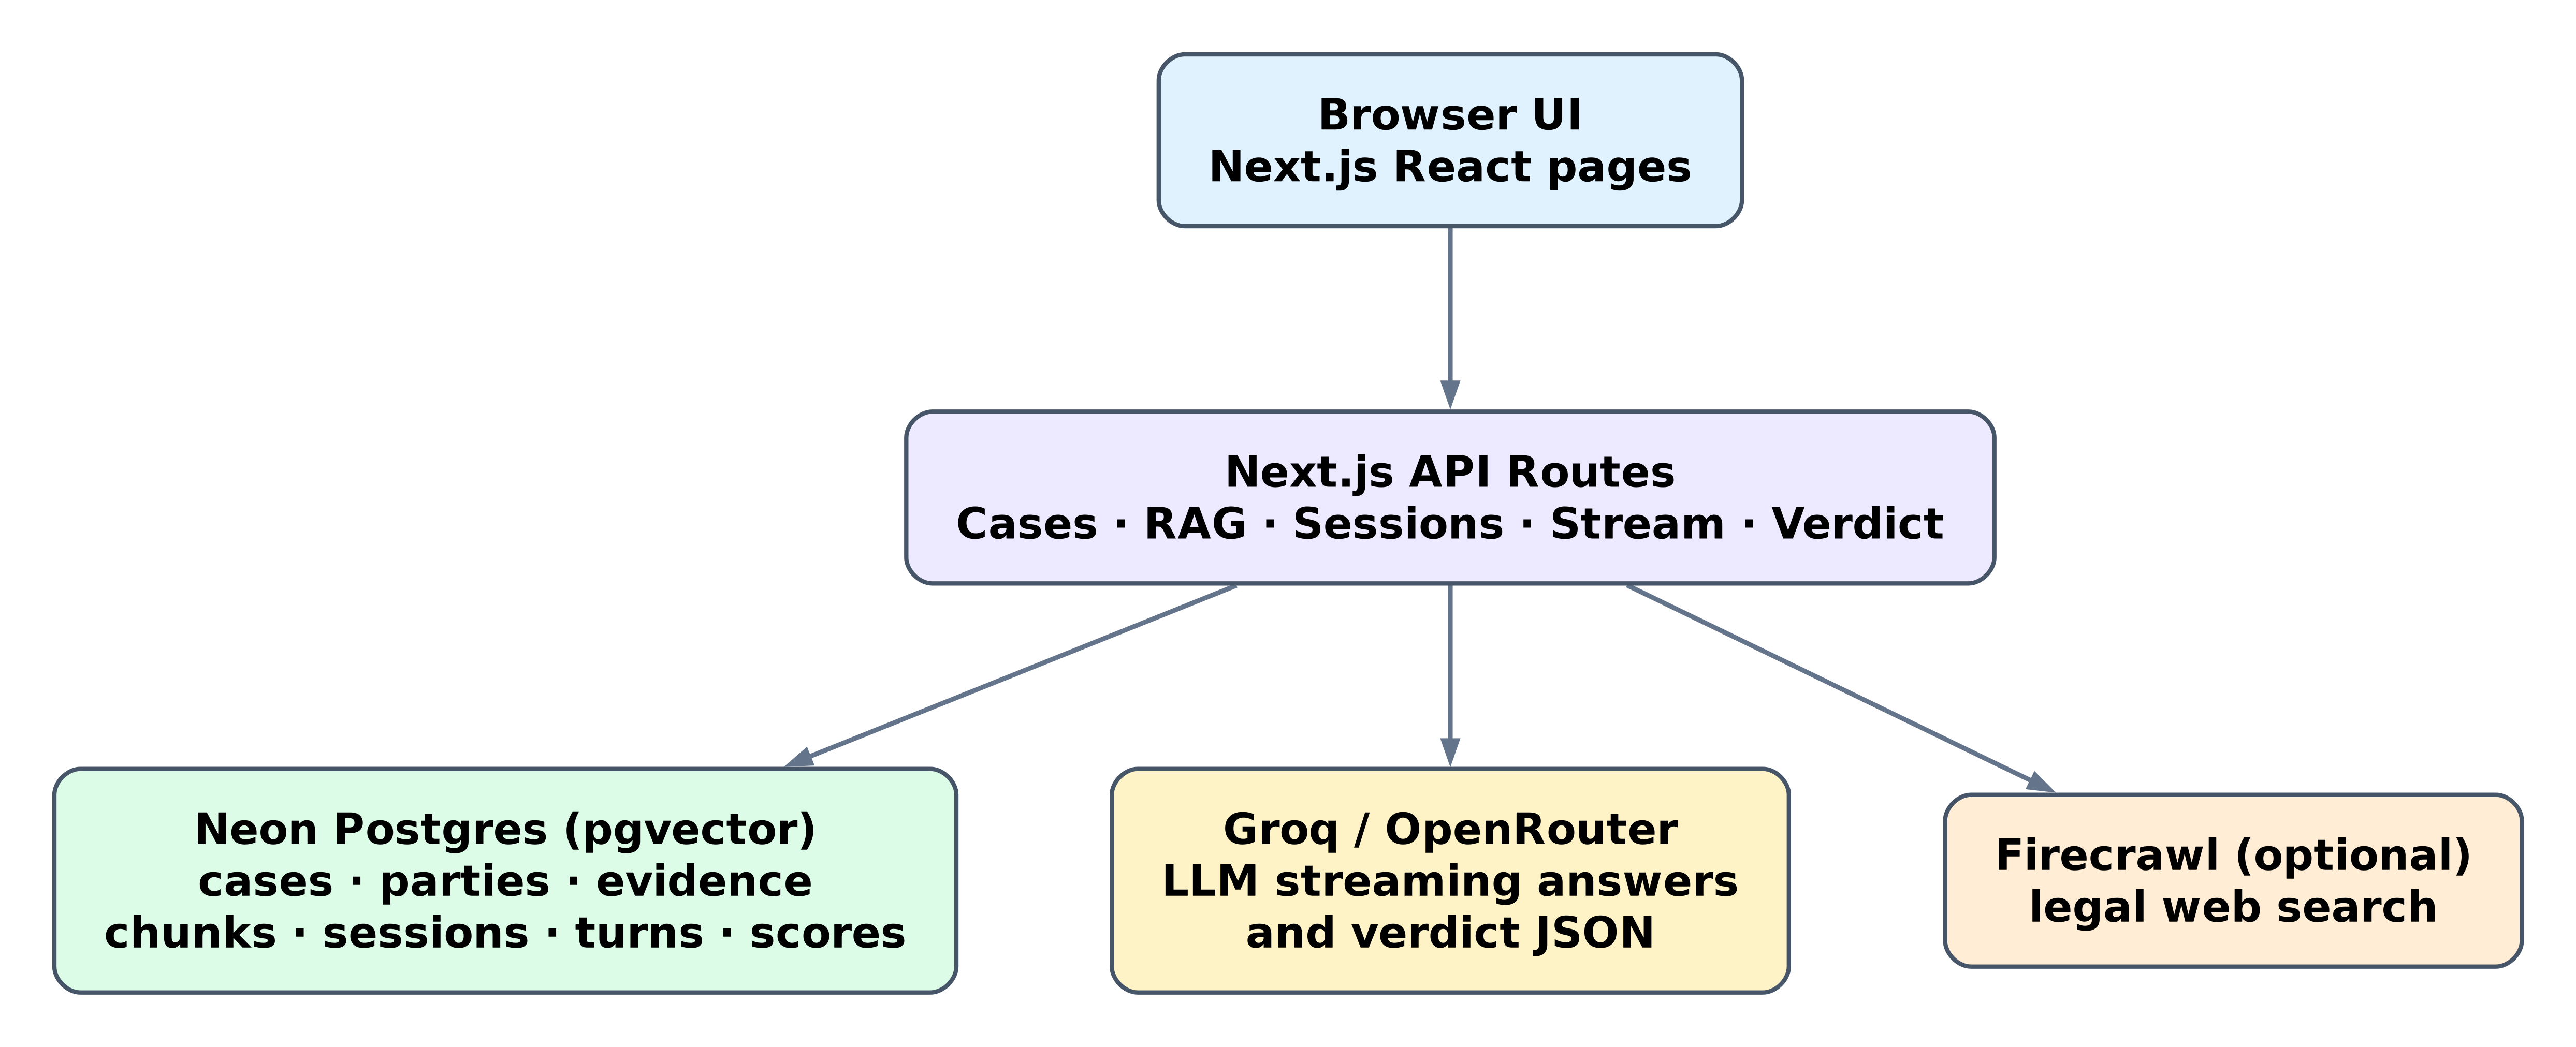
\includegraphics[width=0.98\textwidth]{figures/architecture.png}
\caption{System architecture showing the browser, Next.js API routes, database and AI services.}
\label{fig:architecture}
\end{figure}
 A case has a stable identifier and relates to its evidence and indexed text. A session stores the learner role, duration, status and case identifier. Each dialogue turn is persisted with an actor, speaker, kind, text, citation and sequence number.

\begin{table}[!htbp]\centering\caption{Core data entities used by Courtroom AI.}\label{tab:entities}\begin{tabularx}{0.95\textwidth}{>{\bfseries}p{0.24\textwidth}X}\toprule Entity & Purpose \\ \midrule Cases & Title, court, category, charges and summary for a legal matter. \\ Case parties & Judge, counsel and witness personas used by the simulator. \\ Case evidence & Exhibits with labels, descriptions and case-specific content. \\ Chunks & Section-labelled text passages used by the RAG retriever. \\ Sessions & Learner role, case, duration, status and outcome. \\ Session turns & Ordered student, judge and witness transcript entries. \\ Scores & Argument, objection, composure, legal accuracy and overall feedback. \\ \bottomrule\end{tabularx}\end{table}


\subsection{Legal Judgment Reference Corpus}
Three landmark 2024 Supreme Court of India judgments were ingested verbatim from official sources to anchor retrieval quality. Each is stored as a separate document with section labels that preserve its paragraph structure.

\begin{table}[!htbp]
\centering
\caption{Landmark 2024 judgments ingested as legal-reference documents.}
\label{tab:judgments}
\begin{tabularx}{0.95\textwidth}{p{0.30\textwidth}p{0.13\textwidth}p{0.18\textwidth}X}
\toprule
Judgment & Citation & Bench & Retrieval role \\
\midrule
Sita Soren v. Union of India & 2024 INSC 161 & 7-Judge (CJI Chandrachud) & Articles 105(2), 194(2); bribery and legislative immunity; overrules *P.V. Narasimha Rao*. \\
Bilkis Yakub Rasool v. Union of India & 2024 INSC 24 & 2-Judge (Nagarathna, Bhuyan) & Remission of life sentences (CrPC §§432--433), appropriate government. \\
Sukanya Shantha v. Union of India & 2024 INSC 753 & 2-Judge (CJI Chandrachud, Pardiwala) & Caste-based prison discrimination; Articles 14, 15, 17, 21. \\
\bottomrule
\end{tabularx}
\end{table}

The corpus now totals 914 indexed chunks across five primary documents: the two seeded simulation cases (12 chunks) and the three judgments (902 chunks). All 914 chunks carry active 4096-dimensional embeddings.

\subsection{Demonstration Cases}
The first case is a criminal and corruption matter concerning the 2021--22 Delhi Excise Policy and related CBI/ED proceedings. The second is the constitutional challenge to the Electoral Bonds Scheme, decided in 2024 INSC 113. Both cases are represented by a case summary, parties, evidence exhibits and indexed fact/statute chunks.
\begin{table}[!htbp]\centering\caption{Real cases used in the short demonstration.}\label{tab:cases}\begin{tabularx}{0.95\textwidth}{p{0.29\textwidth}p{0.20\textwidth}X}\toprule Case & Area & Preparation focus \\ \midrule State v. Arvind Kejriwal & Criminal and corruption & Conspiracy, electronic records, money laundering, summons chronology and bail orders. \\ Association for Democratic Reforms v. Union of India & Constitutional law & Article 19(1)(a), political funding transparency, donor privacy and statutory amendments. \\ \bottomrule\end{tabularx}\end{table}


\subsection{Data Preparation and Schema Design}
The two demonstration cases are represented as structured seed records. Each record contains a stable identifier, title, legal category, court, charges and a summary. Party records define the judge, counsel and witness roles. Evidence records define exhibits, descriptions and content. The fact sheet is converted into chunks with section labels such as a constitutional article, statutory provision or case fact. This makes the case usable both as visible preparation material and as retrievable context.


\begin{figure}[!htbp]
\centering
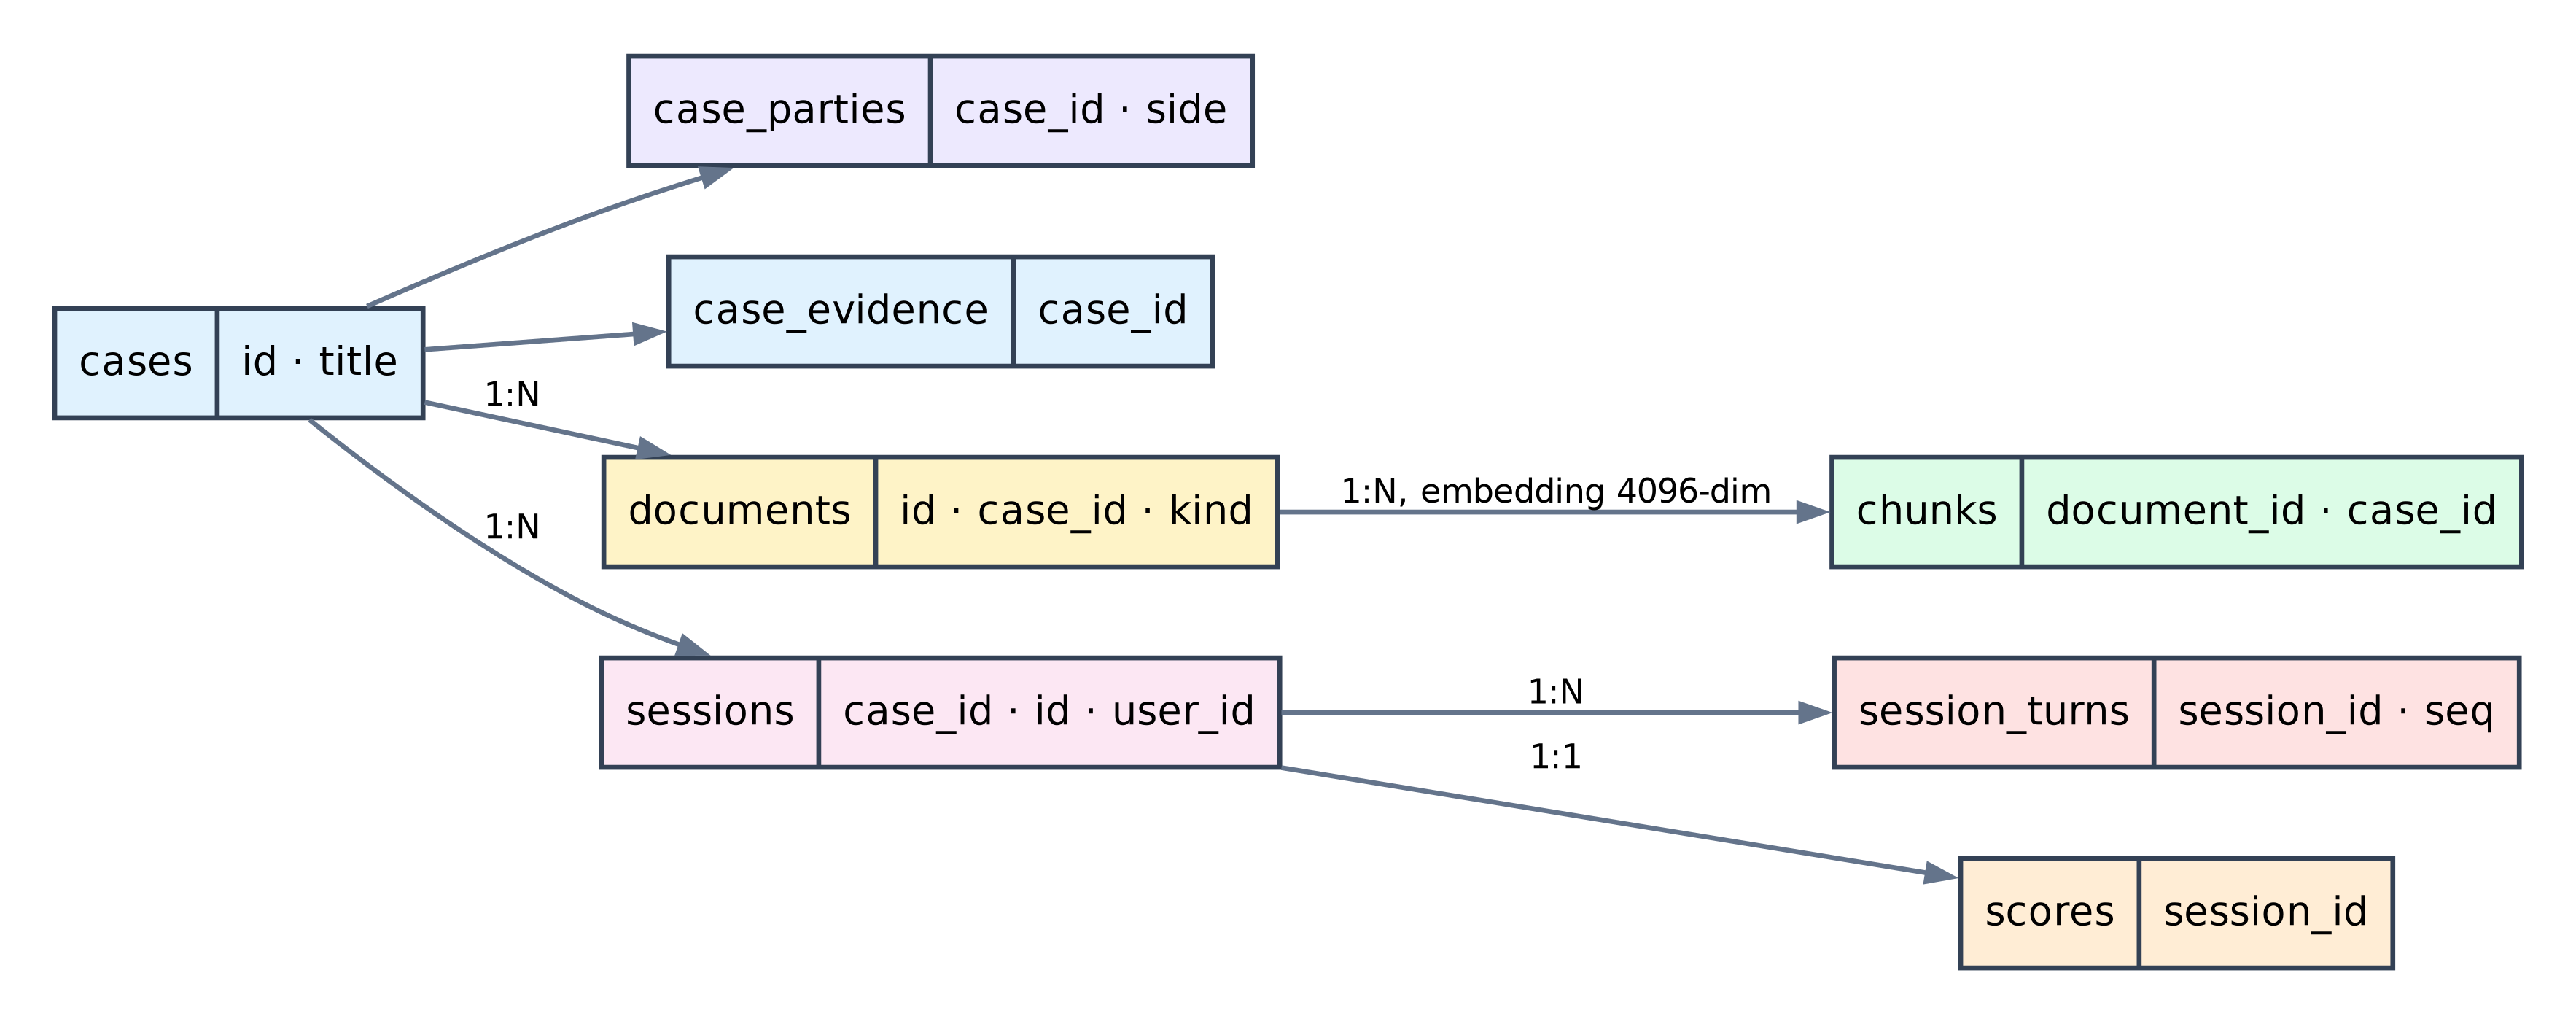
\includegraphics[width=0.98\textwidth]{figures/er-diagram.png}
\caption{Simplified relationship diagram for the persistent project data.}
\label{fig:er}
\end{figure}

The schema is relational because the entities have clear ownership and lifecycle relationships. A case has many parties, exhibits, documents and chunks. A session belongs to one case and has many turns. A score belongs to one session. The session identifier is used at the API boundary, while the case identifier is used to scope retrieval. This separation prevents a research query from unintentionally mixing one case with another.

\subsection{Hybrid Retrieval Algorithm}
The RAG implementation follows the procedure below:
\begin{enumerate}[label=\arabic*.]
\item Normalize the question and retain meaningful terms longer than two characters, removing stopwords and preserving section tokens such as \texttt{§ 61(2)}.
\item Embed the question with \texttt{qwen/qwen3-embedding-8b} via OpenRouter (4096 dimensions). A query-instruction prefix (``Instruct: $\ldots$'') was A/B tested in the ablation and is not applied: it produced no reliable improvement on paired against the plain-query baseline.
\item If a valid vector is available, search chunks with pgvector cosine distance. Playable-case queries are now executed under the \texttt{case-or-null} predicate (\texttt{case\_id = X OR case\_id IS NULL}) so that the three judgment documents created with \texttt{case\_id IS NULL} are reachable; before this fix, the production path returned zero judgment chunks to every case page.
\item Compute a keyword score from the fraction of question terms appearing in the chunk text. This is a naive unigram measure with no stopword handling; measured behaviour of the keyword channel is reported only for reference, since the vector channel carries the recall.
\item Re-rank the top-10 vector candidates with a weighted blend $S(p,q) = 0.4\,K(p,q) + 0.6\,C(p,q)$ and keep the best six.
\item If vector retrieval is unavailable, load case-scoped chunks and rank them using the keyword score. The keyword fallback remains important for offline operation and for trains of API failure.
\item Return up to six passages and insert them into the answer prompt.
\end{enumerate}


\begin{figure}[!htbp]
\centering
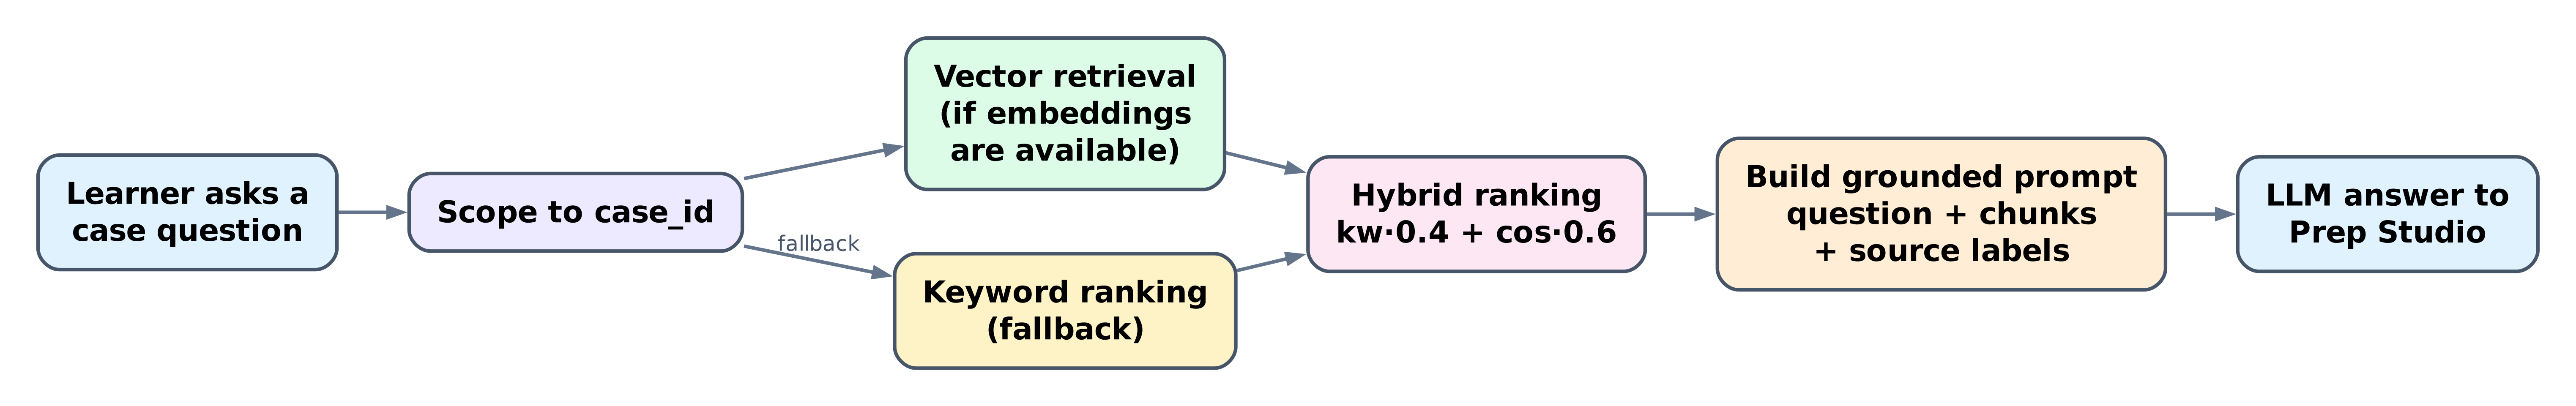
\includegraphics[width=0.98\textwidth]{figures/rag-flow.png}
\caption{Case-scoped hybrid RAG preparation flow.}
\label{fig:ragflow}
\end{figure}

A simplified ranking expression is:
\[
S(p,q) = 0.4 K(p,q) + 0.6 C(p,q),
\]
where $K(p,q)$ is keyword overlap between passage $p$ and question $q$, and $C(p,q)$ is the cosine similarity after clamping it to the interpretable range. In fallback mode, $S(p,q)=K(p,q)$. The fallback remains important for reproducibility and for offline operation. After migration, the vector path returns cosine-distance results from 4096-dimensional Qwen3 embeddings.

\subsection{Embedding Model and Migration}
Embedding generation uses \texttt{qwen/qwen3-embedding-8b} (4096 dimensions) through OpenRouter. The migration from the earlier local nomic text embedding (768 dimensions) proceeded in three steps:\\
(1) the database column was altered to \texttt{vector(4096)} and the affected index recreated, (2) legacy 768-dimensional vectors were nullified to prevent mixed-model retrieval, and (3) the full corpus was re-embedded through the OpenRouter embeddings endpoint with strict 4096-dimension validation. A rollback branch (\texttt{pre-qwen3-backup}) preserves the pre-migration state. All vectors are now homogeneous and produced by the same model.


\subsection{Prompt Construction}
The prompt contains the user question and a clearly delimited list of retrieved passages. The system instruction tells the research assistant to answer only from the supplied sources, cite section labels and state plainly when the sources do not cover the question. The courtroom prompt contains case title, court, charges, summary, exhibits, transcript context and the learner's latest submission. A separate system instruction is selected for judge and witness responses. This role separation prevents a witness from speaking like a judge and makes the transcript easier to interpret.

\subsection{API and Component Design}
The server exposes route handlers for cases, case details, sessions, intros, turns, streaming, verdicts and RAG research. The preparation page calls the case detail and RAG routes. The courtroom page calls session creation and intro routes, and the streaming hook consumes NDJSON responses. The right transcript panel receives the saved transcript plus a temporary streaming item. The component structure therefore mirrors the data flow rather than placing all logic in one page.

\begin{table}[!htbp]
\centering
\caption{Important application endpoints.}
\label{tab:endpoints}
\begin{tabularx}{0.95\textwidth}{p{0.29\textwidth}p{0.16\textwidth}X}
\toprule
Endpoint & Method & Responsibility \\
\midrule
/api/cases & GET & List the two guided demonstration cases. \\
/api/cases/[id] & GET & Return case, parties, evidence and chunks. \\
/api/rag/ask & POST & Retrieve sources and generate a case-grounded answer. \\
/api/sessions & POST & Create a timed practice session. \\
/api/sessions/[id]/intro & POST & Persist the opening judge turn. \\
/api/sessions/[id]/stream & POST & Stream reasoning, deltas and final AI turn. \\
/api/sessions/[id]/verdict & POST & Score the transcript and end the session. \\
\bottomrule
\end{tabularx}
\end{table}

\subsection{Session State Machine}
The intended session states are OPENING, EXAMINATION, OBJECTION, RULING, ARGUMENT, CLOSING and VERDICT. The opening route creates the initial judge turn. A standard learner submission is routed to a witness or judge response. An objection is routed to a judge ruling. A verdict request closes the session and records the score. The status field and end timestamp provide a persistent boundary between a live and completed session.

\subsection{Security and Privacy Considerations}
LLM and database credentials are read from server-side environment variables and are not sent to the browser. Session routes compare the stored session owner with the current user identity; the development fallback uses a guest identity for the local demo. Case-specific retrieval is enforced in the database query. Input text is trimmed and capped before being included in prompts. The system should still be deployed with real authentication, rate limiting, audit logging and a policy for handling uploaded documents before being used with private legal material.

\subsection{Scope and isolation}
\texttt{case-or-null} now means that judgments are reachable from the case pages — this was not the case before the retrieval-layer fix. That said, full matter-versus-matter isolation is deliberately not enforced for judgments, because both playable cases share the same reference corpus. What is enforced is case-to-case isolation between the two simulation cases: Delhi-case queries do not return Electoral Bonds chunks, and vice versa, verified by the regression test T1 (\texttt{scripts/regression-tests.mjs}). The implementation cannot distinguish ``relevant'' from ``irrelevant'' judgment chunks, so a Sita Soren query from the Delhi page will return Sita Soren paragraphs mixed with BNS/PMLA/Aw Adhiniya provisions. That is true in production and is not hidden in this report.

\subsection{Courtroom Interaction and Streaming}
A learner selects a role, either defence counsel or public prosecutor, and selects a duration. The session begins with a judge opening turn. Text submitted to the judge or witness is sent to a streaming endpoint. The server calls the configured provider with streaming enabled and emits newline-delimited events: reasoning steps, text deltas and a final persisted turn. The client reads these events as they arrive. Each delta updates the temporary transcript item, so the response appears progressively on the right side rather than arriving as one delayed block.


\begin{figure}[!htbp]
\centering
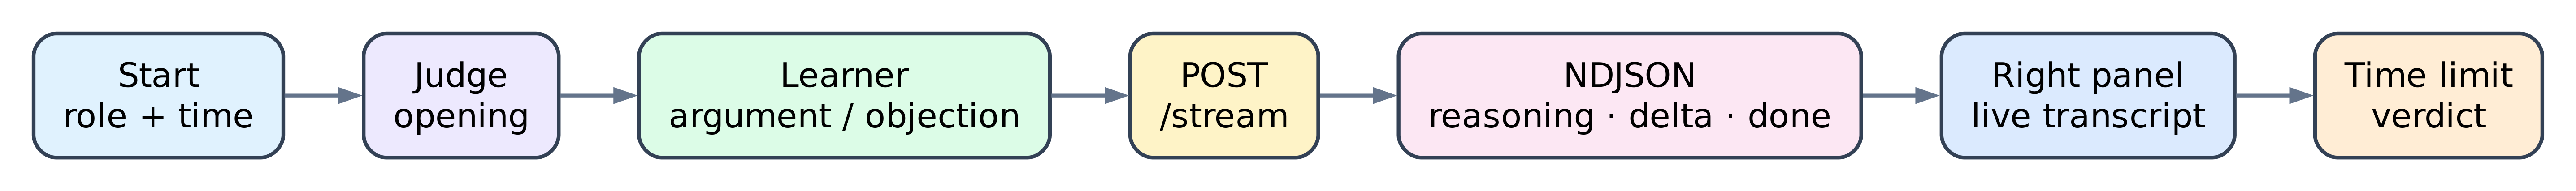
\includegraphics[width=0.98\textwidth]{figures/stream-flow.png}
\caption{Timed courtroom and real streaming flow from session start to verdict.}
\label{fig:streamflow}
\end{figure}

Objection buttons use the same stream endpoint with an objection kind. The judge prompt is instructed to begin with a ruling such as ``OBJECTION SUSTAINED'' or ``OBJECTION OVERRULED'' and to provide a short reason.

\subsection{Time-Bound Session Control}
The selected duration is stored in the session record. The client displays elapsed time and automatically requests a verdict when the limit is reached. The server independently checks the session start time and duration before accepting intro, turn, advance or stream requests. An expired session is marked ended with an end timestamp and new interaction requests receive a conflict response.

\subsection{Verdict Evaluation}
At the end of the session, the verdict route sends the persisted transcript and case context to an evaluation prompt. The response is parsed as structured JSON and stored in the scores table. The report contains argument score, objection score, composure score, legal accuracy score, an overall score, judge summary, strengths and weaknesses.

\begin{figure}[t]
\centering
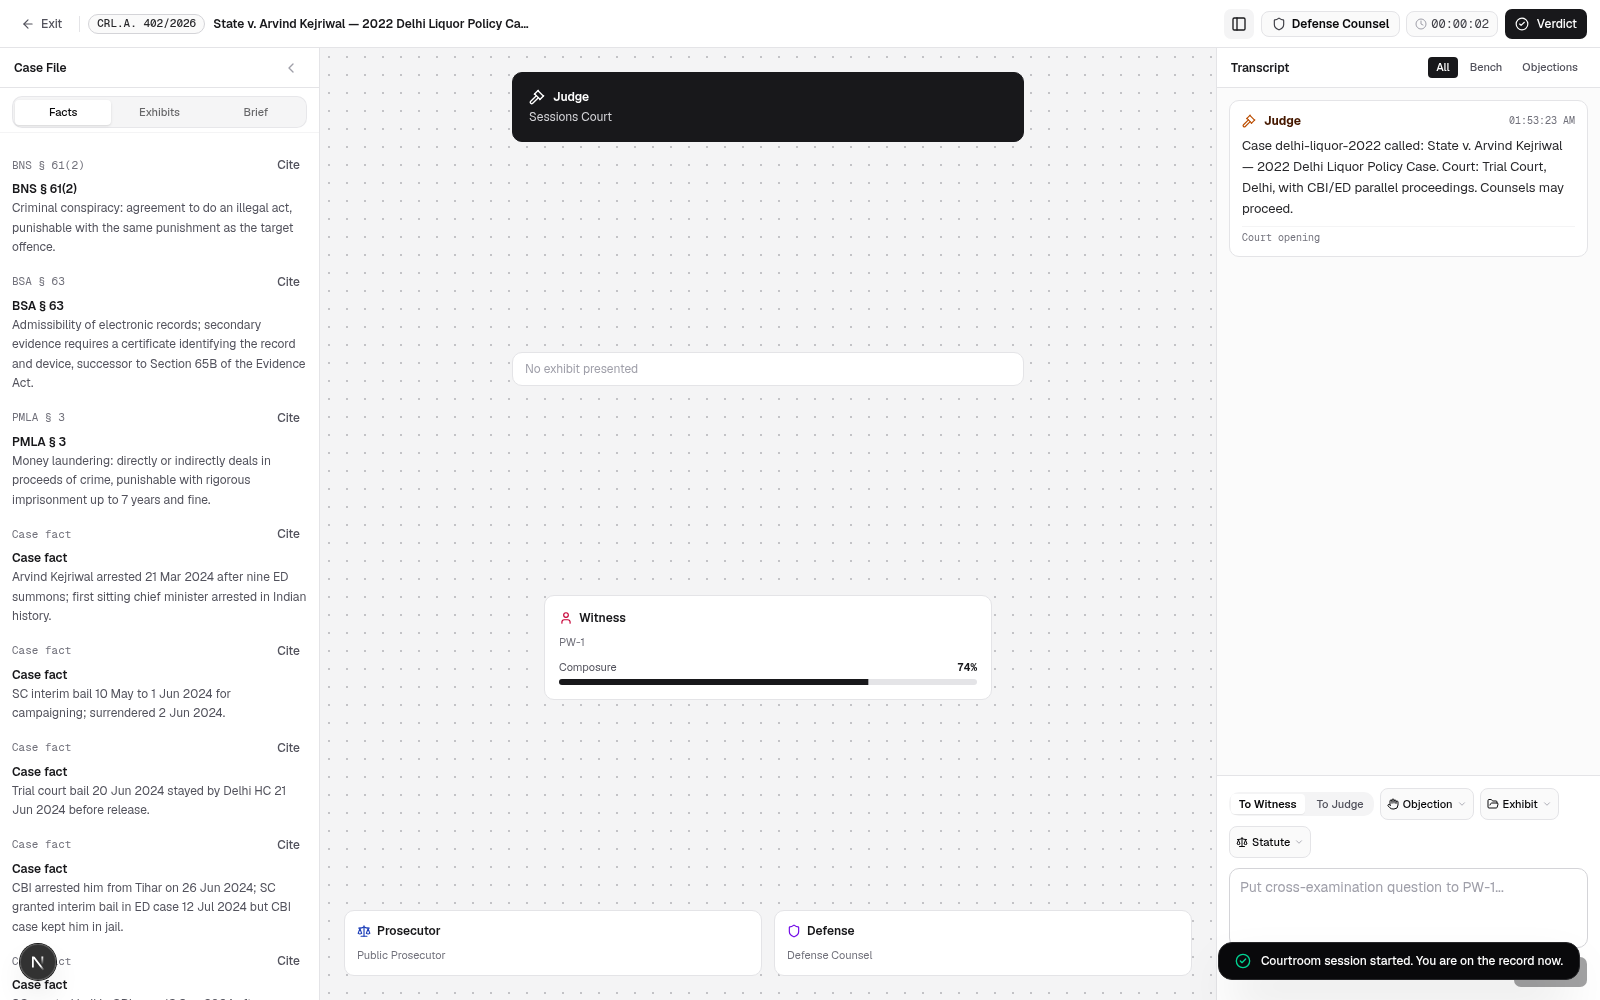
\includegraphics[width=0.98\textwidth]{figures/courtroom-arena.png}
\caption{Three-pane courtroom interface for the Delhi case: Case File dossier (left), courtroom arena (center), and Transcript/Advocate Console (right). The opening judge turn is persisted and rendered in the right panel.}
\label{fig:arena}
\end{figure}

\begin{figure}[t]
\centering
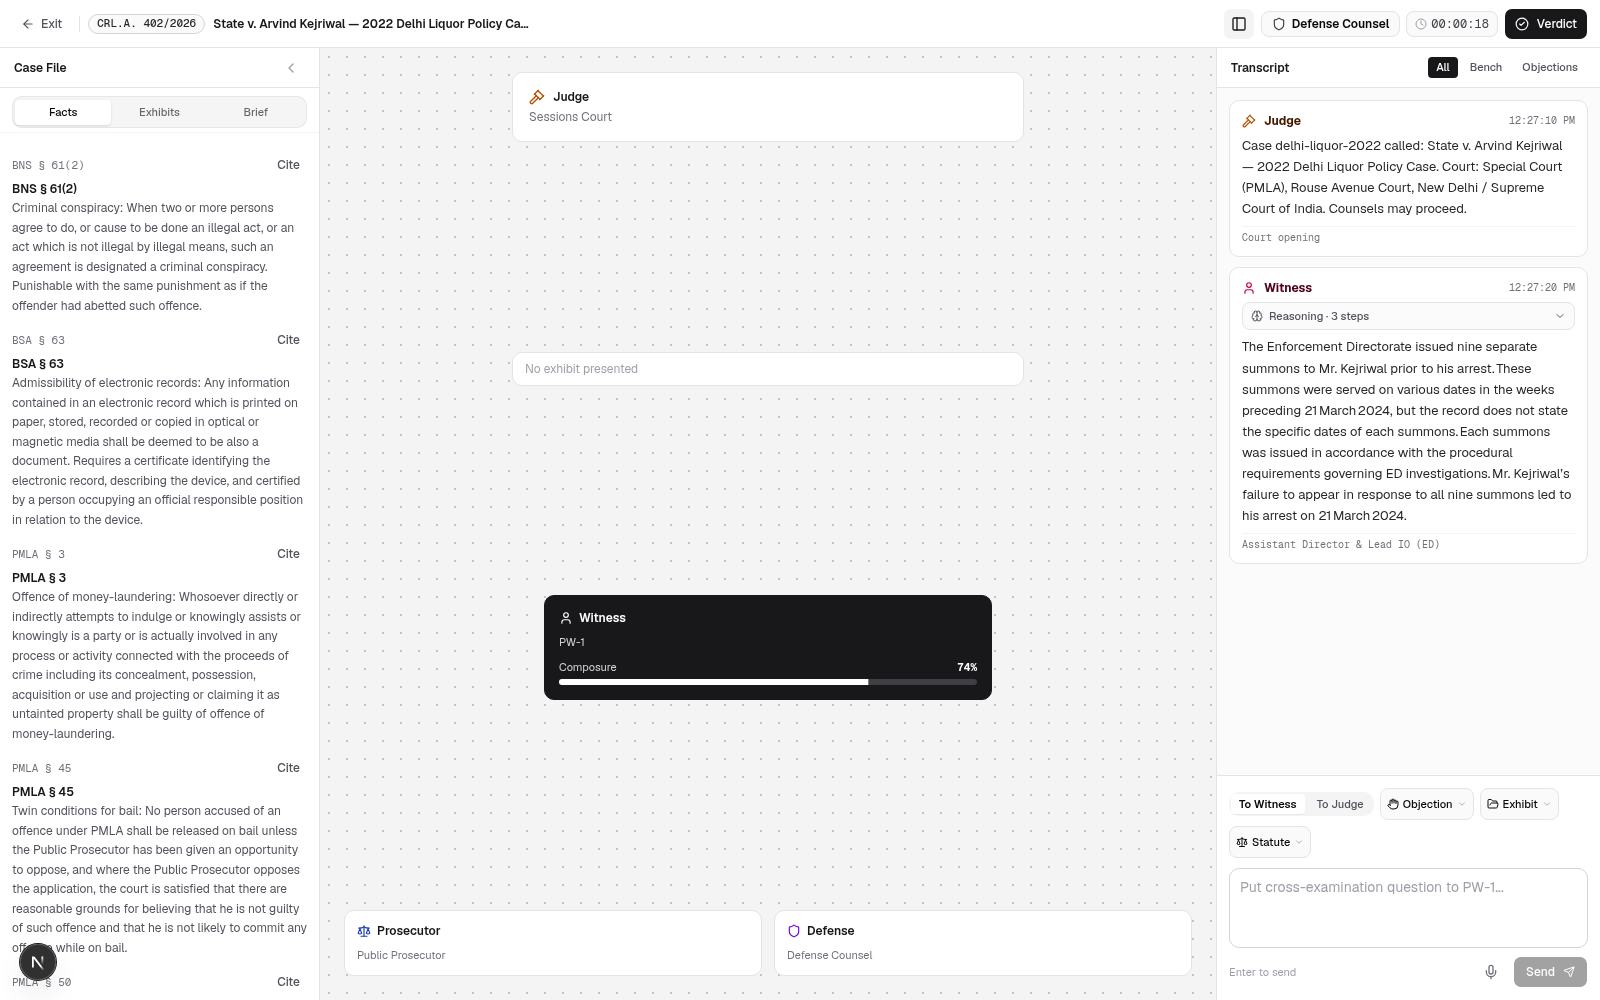
\includegraphics[width=0.98\textwidth]{figures/courtroom-streaming.png}
\caption{Right-hand transcript panel during a live streamed witness response. The witness states nine summons and the arrest date, and expressly says the record does not state the individual dates --- the behaviour produced by the grounding prompt and the runtime grounding check of \S4.4.}
\label{fig:streaming}
\end{figure}

\section{Results and Discussions}
\subsection{Functional Results}
The application was tested using the two guided cases. For each case, the sequence was exercised: case listing, case detail loading, RAG question, session creation, judge intro, streamed learner turn and verdict generation. The responses confirmed that case data and session records were available, the stream produced a final completion event and the verdict was persisted.
\begin{table}[!htbp]\centering\caption{End-to-end demonstration checks.}\label{tab:results}\begin{tabularx}{0.95\textwidth}{p{0.36\textwidth}ccX}\toprule Check & Delhi case & Bonds case & Observation \\ \midrule Case detail and indexed chunks & Pass & Pass & Each case returned case-specific facts and exhibits. \\ RAG question & 200 & 200 & Answers returned ranked case-scoped source labels. \\ Session creation and intro & 201 & 201 & A live session and opening judge turn were persisted. \\ Real streamed courtroom turn & 200 & 200 & Reasoning, delta and done events were received. \\ Verdict generation & 200 & 200 & Score and judge summary were saved. \\ \bottomrule\end{tabularx}\end{table}




\begin{figure}[t]
\centering
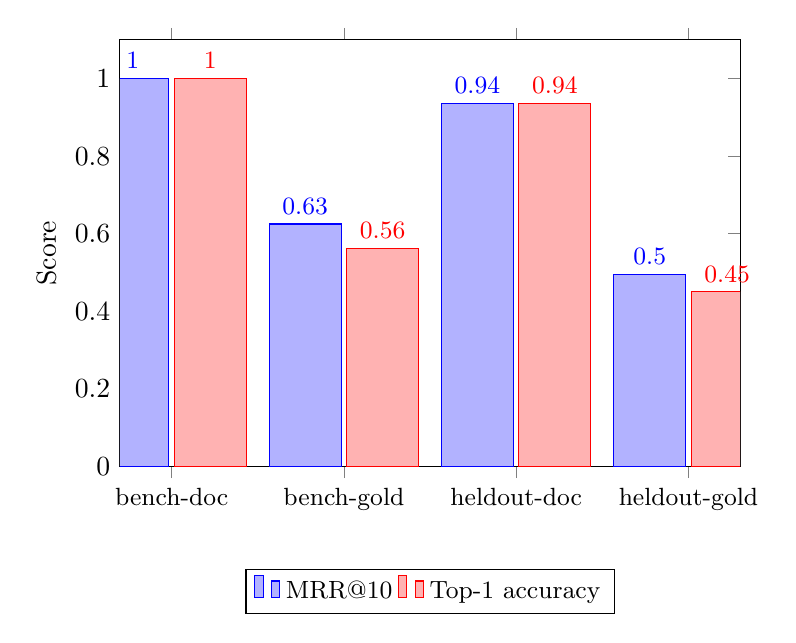
\begin{tikzpicture}
\begin{axis}[
  ybar,
  width=0.78\textwidth,
  height=7cm,
  ymin=0, ymax=1.1,
  ylabel={Score},
  symbolic x coords={bench-doc,bench-gold,heldout-doc,heldout-gold},
  xtick=data,
  x tick label style={font=\small},
  nodes near coords,
  nodes near coords style={font=\small},
  bar width=26pt,
  legend style={font=\small, at={(0.5,-0.24)}, anchor=north, legend columns=2},
]
\addplot coordinates {(bench-doc,1.0000) (bench-gold,0.6250) (heldout-doc,0.9362) (heldout-gold,0.4958)};
\addlegendentry{MRR@10}
\addplot coordinates {(bench-doc,1.0000) (bench-gold,0.5625) (heldout-doc,0.9362) (heldout-gold,0.4500)};
\addlegendentry{Top-1 accuracy}
\end{axis}
\end{tikzpicture}
\caption{Vector-only retrieval measured directly from \texttt{data/eval/ablation\_gold.json}: MRR@10 and top-1 accuracy for the benchmark and held-out question sets, at document level and at gold-chunk (paragraph-anchored) level.}
\label{fig:evalchart}
\end{figure}


\subsection{Legal Retrieval Evaluation}
A curated 30-question benchmark was constructed across the five matters in the corpus, using the question style of IndicLegalQA (PMC12166829) and official Supreme Court texts. The questions cover legislative privilege (Sita Soren), remission and executive power (Bilkis Yakub Rasool), prison reform (Sukanya Shantha), electoral funding (Electoral Bonds) and criminal procedure/admissibility (Delhi Liquor). Each question is paired with its expected judgment, citation and supporting paragraph.

\begin{table}[!htbp]
\centering
\caption{Retrieval ablation, global scope. ``doc'' = right document matter; ``gold'' = right document plus paragraph anchor overlap (Jaccard$\ge$0.5), computed only over questions with a non-empty gold set.}
\label{tab:eval}
\begin{tabularx}{0.95\textwidth}{p{0.20\textwidth}p{0.17\textwidth}p{0.20\textwidth}p{0.10\textwidth}p{0.11\textwidth}}
\toprule
Ranker & Metric & Set (n) & MRR@10 & Top-1 \\
\midrule
vector-only     & doc  & bench (30)   & 1.000 & 1.000 \\
hybrid-0.2/0.8  & doc  & bench (30)   & 1.000 & 1.000 \\
hybrid-0.4/0.6 & doc  & bench (30)   & 1.000 & 1.000 \\
hybrid-0.6/0.4 & doc  & bench (30)   & 0.983 & 0.967 \\
keyword-only    & doc  & bench (30)   & 0.600 & 0.600 \\
\midrule
vector-only     & gold & bench (16)   & 0.625 & 0.562 \\
hybrid-0.2/0.8  & gold & bench (16)   & 0.645 & 0.625 \\
hybrid-0.4/0.6 & gold & bench (16)   & 0.645 & 0.625 \\
hybrid-0.6/0.4 & gold & bench (16)   & 0.614 & 0.562 \\
keyword-only    & gold & bench (16)   & 0.563 & 0.562 \\
\midrule
vector-only     & doc  & held-out (47) & 0.936 & 0.936 \\
hybrid-0.2/0.8  & doc  & held-out (47) & 0.926 & 0.915 \\
hybrid-0.4/0.6 & doc  & held-out (47) & 0.915 & 0.894 \\
hybrid-0.6/0.4 & doc  & held-out (47) & 0.910 & 0.894 \\
keyword-only    & doc  & held-out (47) & 0.560 & 0.532 \\
\midrule
vector-only     & gold & held-out (20) & 0.496 & 0.450 \\
hybrid-0.2/0.8  & gold & held-out (20) & 0.482 & 0.450 \\
hybrid-0.4/0.6 & gold & held-out (20) & 0.482 & 0.450 \\
hybrid-0.6/0.4 & gold & held-out (20) & 0.457 & 0.400 \\
keyword-only    & gold & held-out (20) & 0.450 & 0.450 \\
\bottomrule
\end{tabularx}
\end{table}

A short 30-question benchmark was constructed across the five matters, question style derived from IndicLegalQA and official Supreme Court texts; the questions cover legislative privilege (Sita Soren), remission and executive power (Bilkis Yakub Rasool), prison reform (Sukanya Shantha), electoral funding (Electoral Bonds) and criminal procedure/admissibility (Delhi Liquor). Each question is paired with its expected judgment and citation.

Relevance is defined three ways and measured for every cell: (1) lenient (citation substring match), (2) document-level (right document matter), (3) strict (right document AND Jaccard$\ge$0.5 between chunk text and anchor passage; degrades to document-level when the anchor does not exist — the common case for Bilkis, Sukanya and Electoral Bonds, whose chunks carry no explicit paragraph labels).

The bench-set Table above is the current \texttt{data/eval/ablation\_gold.json} output, produced by \texttt{node scripts/ablation-gold.mts}. Gold metrics are shown for the subset of questions whose gold chunk set is non-empty; deriving gold-flex is a separate, stricter exercise than the report claims were known before.

The figures for the held-out set differ systematically from the benchmark (because they were phrased to avoid lexical overlap): the MRR slips from 1.00 to 0.92, the right-document hit rate from 100\% to 93.6\%. That gap reflects the lexical-similarity cheating the benchmark allowed and is the principal reason the held-out set was added.

The Qwen3 query-instruction prefix was A/B tested and is not applied (see \S4.2): it did not improve the paired deltas. Keyword-only is materially worse across every metric.

Per-ranker differences are small (one question moves the MRR by $\pm0.03$). With $n=30$, differences between the three hybrid weightings are noise; any of them, or none, would produce a similar table. Only keyword-only is unambiguously worse.

\subsection{Faithfulness and Grounding Evaluation}
Before the grounding work, the witness turn invented nine dated summons, a diary entry (``Diary entry 21-03-2024, Para 12'') and a statutory reference (Section 65B of the Indian Evidence Act, 1872 --- the corpus holds BSA \S63). The judge turn imported ``Section 65B of the Information Technology Act, 2000'', a statute that is nowhere in the corpus. The Witness Lab was worse: that route supplied the persona with no case record at all, so it answered ``two summons ... 15 January 2022'' --- wrong count and wrong year.

Three changes address this. First, the witness and judge prompts now state that only the case brief may be used and that a missing specific must be answered with ``the record does not state that''. Second, the Witness Lab route was given the case record (all exhibits and fact chunks) instead of nothing. Third, and most importantly, a deterministic grounding check (\texttt{src/lib/grounding.ts}) extracts the concrete artifacts a turn asserts --- dates, section and article numbers, diary and page references, numeric counts --- and tests each against the text actually supplied to the model. A turn that fails is regenerated once with the offending item named; if it still fails, it is replaced by a refusal to state what the record does not contain. This is a runtime control, not a prompt convention.

\begin{table}[!htbp]
\centering
\caption{Invented-specifics scan on the final build (\texttt{data/eval/specifics\_scan.json}). Eight detail-probing turns across both playable cases, checked with the same module the application uses at runtime.}
\label{tab:specifics}
\begin{tabularx}{0.86\textwidth}{>{\bfseries}p{0.26\textwidth}cccX}
\toprule
Turn type & Turns & Violations & Clean & Example (grounded answer) \\
\midrule
witness & 5 & 0 & 5 & ``The record does not state the exact dates on which each electoral bond was issued and purchased.'' \\
judge & 3 & 0 & 3 & ``Objection sustained. The record contains the Election Commission's counter-affidavit (Exhibit F).'' \\
\midrule
Total & 8 & 0 & 8 & \\
\bottomrule
\end{tabularx}
\end{table}

The claim-level faithfulness harness (\texttt{scripts/eval-faithfulness.mts}) was then run against the final build. Answers are classified as an answer or an abstention before scoring, abstention sentences are excluded from the claim pool, and questions whose split or judge output failed are counted rather than dropped.

\begin{table}[!htbp]
\centering
\caption{Faithfulness on the final build (20 questions, \texttt{data/eval/faithfulness.json}).}
\label{tab:faith}
\begin{tabularx}{0.92\textwidth}{>{\bfseries}p{0.5\textwidth}X}
\toprule
Measure & Value \\
\midrule
Questions asked & 20 \\
Classified as abstention & 2 (10.0\%) \\
Classified as answer & 18 \\
Questions with scoreable claims & 5 \\
Questions that failed split or judge & 13 \\
Total claims judged & 24 \\
Claims supported & 22 (91.7\%) \\
Claims unsupported & 2 (8.3\%) \\
Claims contradicted & 0 \\
Generation model & \texttt{openai/gpt-oss-120b} \\
Judge model & \texttt{openai/gpt-oss-20b} \\
\bottomrule
\end{tabularx}
\end{table}

Three caveats are recorded rather than smoothed over. The judge comes from the same vendor as the generator. Thirteen of twenty questions produced no scoreable claims, mostly because the answer was an abstention the splitter could not decompose into atomic claims, so the headline percentage rests on five questions and twenty-four claims. And the harness itself is stochastic: the same twenty questions scored 77.4\% before the grounding changes, 96.0\% after the prompt change alone, and 91.7\% on the final build --- a spread of roughly nineteen points driven by which questions happen to yield scoreable claims, which is itself a reason to treat the figure as indicative rather than precise.

\clearpage
\subsection{Fixes and their Measured Effect}
Six changes were applied during this session. Each row states the measured behaviour before the change and the measured behaviour after it. The ``before'' column is taken from the failing output captured in the session log and the ``after'' column from a rerun of the same request against the fixed build. Two rows concern the retrieval layer, three concern generated courtroom content, and one concerns the verdict rubric.
\begin{table}[H]
\centering
\small
\caption{Fixes applied this session. ``Before'' and ``after'' are measured from the same live endpoint reruns.}
\label{tab:fixes}
\begin{tabularx}{0.98\textwidth}{p{0.27\textwidth}p{0.33\textwidth}p{0.30\textwidth}}
\toprule
Fix & Before & After \\
\midrule
Null-scope retrieval fix & A query without a case identifier returned zero judgment chunks; the keyword fallback returned Delhi chunks for any question & The same question from the Delhi page now returns Sita Soren chunks; case-to-case isolation still holds (T1) \\
Embedding migration (pre-existing) & 768-dimensional nomic index & 914 of 914 chunks at 4096 dimensions; no NULL embeddings \\
Grounding prompts for witness and judge & Nine dated summons, a fictional diary entry and Section 65B before the fix & Answers now defer to the record for missing specifics \\
Runtime grounding check & Not implemented; invention depended on prompt wording alone & Eight detail-probing turns checked against the record: 0 violations; failing turns are regenerated once, then withheld \\
Witness Lab case record & The persona received no exhibits or facts and answered ``two summons ... 15 January 2022'' & The record is supplied to the persona; the answer quotes Exhibit A and refuses to add dates \\
Verdict temperature 0.3 $\rightarrow$ 0 & 2 of 5 runs returned no scores & 0 of 5 runs failed to parse; scores still range 5--8 on identical input \\
Index check & not previously checked & No ANN index exists; the table is scanned sequentially; improvement deferred \\
\bottomrule
\end{tabularx}
\end{table}
\FloatBarrier

\subsection{Fixes that Were Not Applied}
Four candidate improvements were measured or scoped and deliberately not applied.
\begin{itemize}
\item \textbf{Hybrid weight retune.} Measured. The differences between the three hybrid weightings on the 30-question benchmark move the MRR by roughly $0.03$ and are driven by a single question, so no change was made.
\item \textbf{Query instruction prefix for qwen3-embedding.} A/B tested with the prefix-ablation script. There was no consistent win: held-out gold MRR improved from 0.496 to 0.549 for vector-only, but the case-scoped hybrid-0.4/0.6 configuration regressed sharply (MRR 0.43 to 0.20). The prefix therefore remains an opt-in parameter that the application does not set.
\item \textbf{Retriever with an explicit reranker.} Would require a new paid API dependency and was deferred pending authorisation.
\item \textbf{Halfvec(4096) HNSW index.} A candidate for approximate-nearest-neighbour retrieval. Stock pgvector caps \texttt{hnsw} at 2000 dimensions, so a 4096-dimensional vector column would need either the \texttt{halfvec} storage type or a dimension reduction, neither validated at this corpus size.
\end{itemize}

\subsection{Testing Methodology}
Testing was performed at three levels. First, build verification checked that the Next.js application compiled and TypeScript page data was valid. Second, API smoke tests exercised case listing, case detail, RAG, session creation, intro, stream and verdict routes. Third, an end-to-end session test repeated the same flow independently for both demonstration cases. The stream was not considered successful merely because it returned status 200; the test also inspected the event types and required the final \texttt{done} event.

A self-hosted regression suite lives at \texttt{scripts/regression-tests.mjs}. 9 of 9 runnable tests passed on this session --- case-scope isolation (Delhi question returns no Electoral Bonds chunks), verdict-schema JSON validity, expired-session conflict, missing-session 404, and stream completion. The one skipped test (wrong-owner access) requires a second authenticated user, which would require a DB write not authorised in this task.

\begin{table}[!htbp]
\centering
\caption{Regression suite actually executed against the running application. Output is reproduced verbatim in the appendix and re-run on every verification pass.}
\label{tab:testcases}
\begin{tabularx}{0.97\textwidth}{p{0.07\textwidth}p{0.30\textwidth}p{0.11\textwidth}X}
\toprule
ID & Assertion & Result & Observed evidence \\
\midrule
T0 & A session can be created & Pass & HTTP 201 with a session identifier returned. \\
T1 & Case-scope isolation holds & Pass & A Delhi-case query returned no Electoral Bonds chunk; returned labels are Delhi provisions and judgment chunks only. \\
T2a & The opening judge turn is created & Pass & HTTP 201 from \texttt{POST /api/sessions/\{id\}/intro}. \\
T2b & A verdict closes the session & Pass & HTTP 200 from \texttt{POST /api/sessions/\{id\}/verdict}; the session is marked ended. \\
T2c & An ended session rejects further turns & Pass & A second intro on the ended session returned HTTP 409. \\
T3 & A session is unreachable by another user & Skipped & Requires a second authenticated user, which would need a database write that was not authorised. \\
T4 & A missing session is not found & Pass & HTTP 404 for an unknown session identifier. \\
T5 & A streamed turn terminates correctly & Pass & NDJSON event sequence was reasoning, then many delta events, then a final \texttt{done} event. \\
T6 & The verdict is valid structured JSON & Pass & All five rubric fields were numbers within $[0,10]$ in the returned record. \\
T7 & Retrieval returns source labels & Pass & Six non-empty section labels were returned for the query. \\
\midrule
\multicolumn{4}{l}{\textbf{Total executed:} 9 tests, 0 failed, 1 skipped.} \\
\bottomrule
\end{tabularx}
\end{table}

\subsection{Observed Results}
The case API returned the two intended identifiers: \texttt{delhi-\allowbreak liquor-\allowbreak 2022} and \texttt{electoral-\allowbreak bonds-\allowbreak 2024}. The case detail responses contained indexed chunks and evidence for both cases. The tested Delhi-case RAG question returned six source labels (two statutes, one BSA section, three case facts), each grounded in the linked corpus. Both sessions returned HTTP 201 during creation and intro, HTTP 200 for streaming, and HTTP 200 for verdict generation. Each stream contained reasoning events, multiple delta events and a final \texttt{done} event. All captured results are from the current live build; artefacts under \texttt{data/eval/} record the retrieval benchmark.

\subsection{Discussion of the Results}
The results demonstrate that the project is not limited to a static front-end mockup. The case listing is connected to database records, the RAG answer is connected to case chunks, the courtroom response is connected to an upstream streaming model and the verdict is connected to a persisted session transcript. The source labels are especially valuable in a data-science context because they provide a trace from input question to retrieved evidence to generated answer.

The time limit is implemented at two layers. The client timer gives immediate feedback and automatically requests a verdict. The server compares the stored start time with the stored duration before accepting new interactions. This protects the rule even if the browser timer is paused or manipulated. The duplicate timer in the courtroom top bar was removed so that one page-level timer is authoritative.

\subsection{Preparation Interface}
The preparation interface separates the case file from research and witness practice. The case-file tab gives the learner an immediate view of evidence and indexed facts (Figure~\ref{fig:prep-casefile}). The RAG tab gives a focused question-and-answer interaction and identifies the sources used (Figure~\ref{fig:prep-rag}). This is more useful than a generic chatbot because the user can move from a retrieved proposition to the exhibit or fact that supports it. The Witness Lab tab lets the learner coach a persona (PW-1 or DW-1 in the Delhi case) and receives LLM responses in character from that persona (Figure~\ref{fig:witness}).

\begin{figure}[t]
\centering
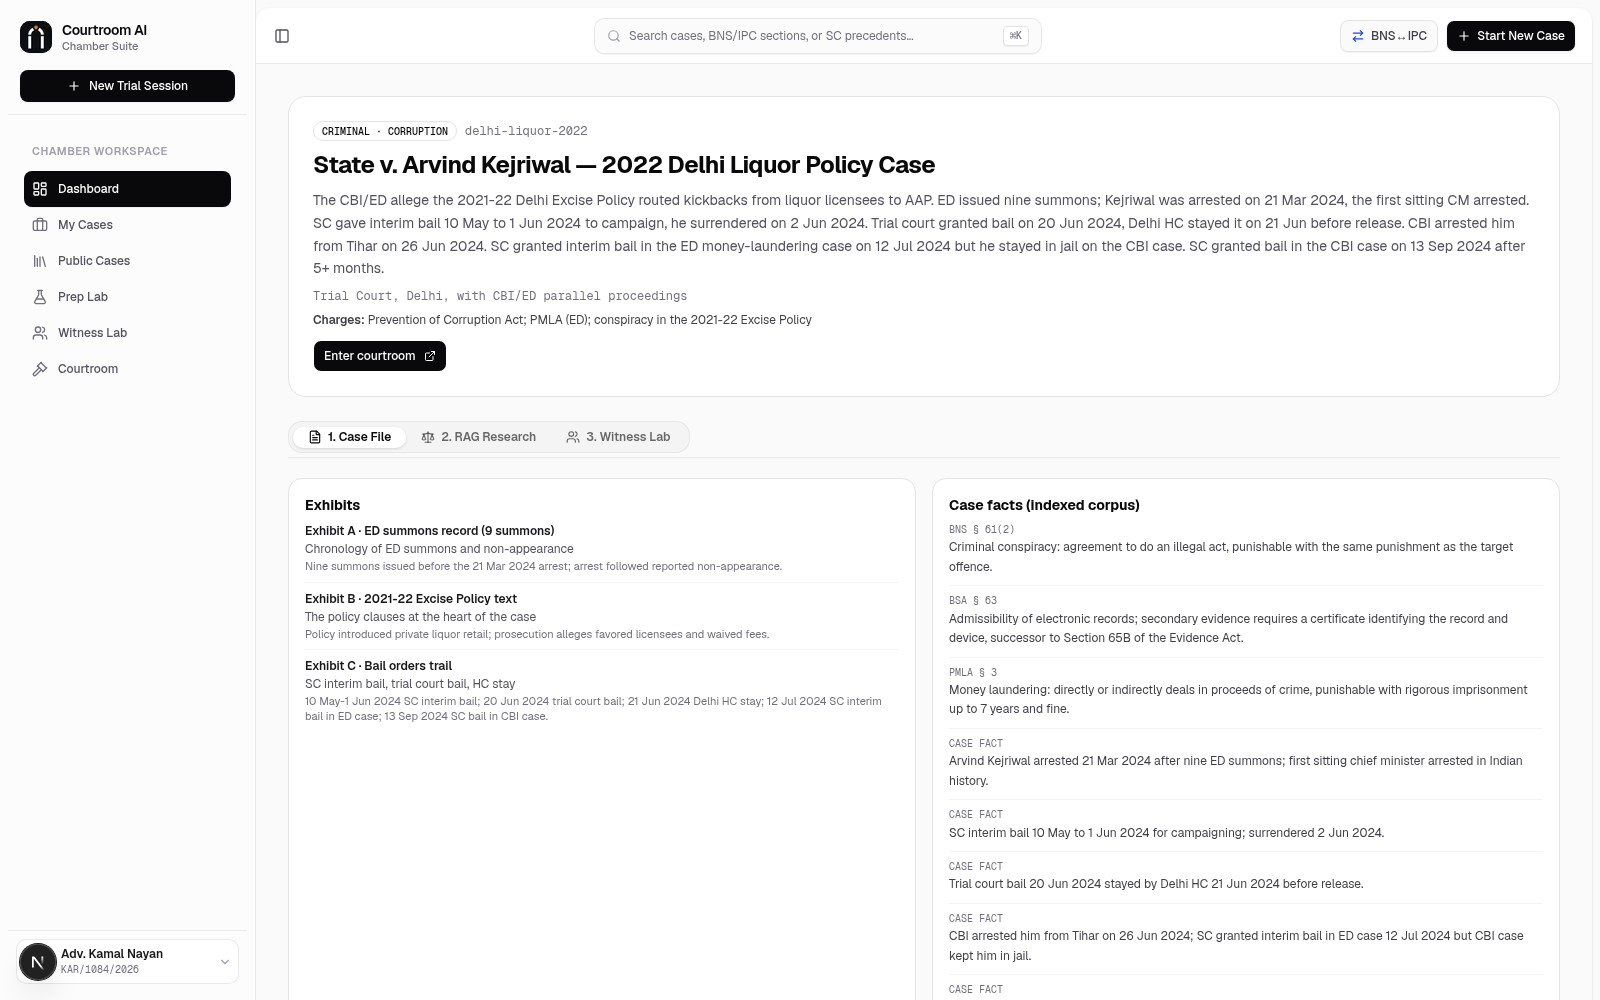
\includegraphics[width=0.98\textwidth]{figures/prep-case-file.png}
\caption{Case File tab for \texttt{delhi-liquor-2022}: exhibits on the left, indexed corpus chunks on the right.}
\label{fig:prep-casefile}
\end{figure}

\begin{figure}[t]
\centering
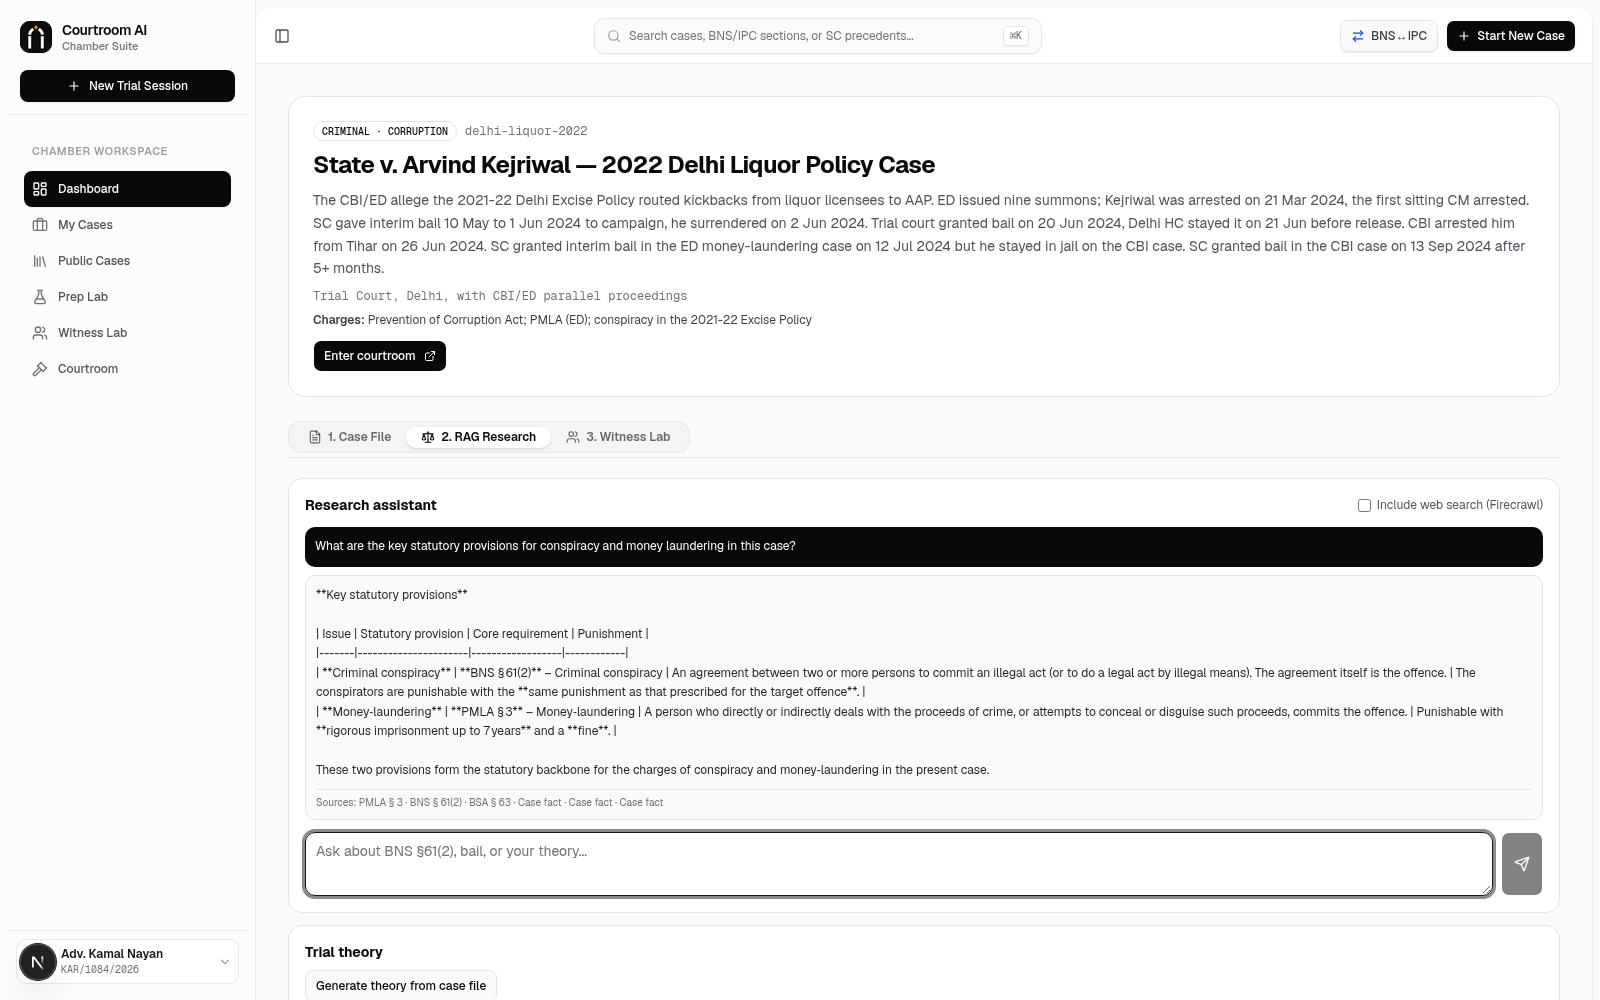
\includegraphics[width=0.98\textwidth]{figures/prep-rag-sources.png}
\caption{RAG Research tab for the Delhi case. Question, retrieved chunks and source labels (BNS \S 61(2), BSA \S 63, PMLA \S 3) are shown.}
\label{fig:prep-rag}
\end{figure}

\begin{figure}[t]
\centering
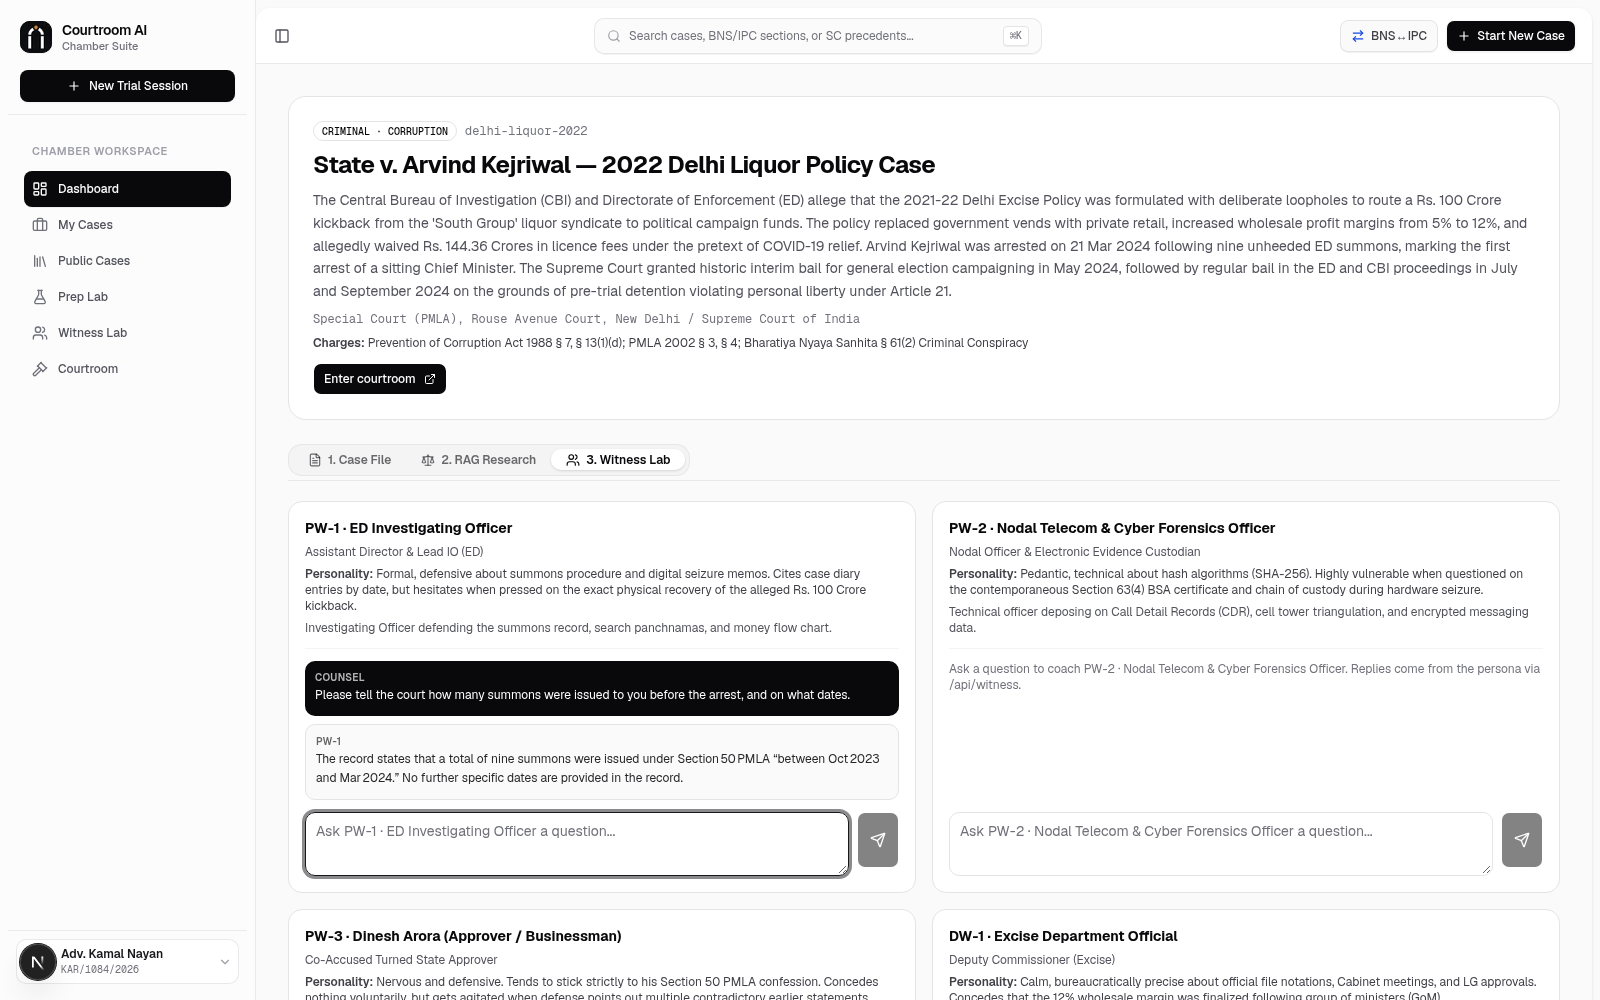
\includegraphics[width=0.98\textwidth]{figures/witness-response.png}
\caption{Witness Lab tab for the Delhi case. Asked for the summons count and dates, the persona replies with what the record contains --- nine summons under Section 50 PMLA between Oct 2023 and Mar 2024 --- and adds that no further specific dates are provided in the record.}
\label{fig:witness}
\end{figure}

\subsection{Courtroom Streaming and Feedback}
The right-side panel is the principal performance surface. It contains the saved transcript and the in-progress streamed response. During a response, reasoning indicators and partial text are visible (Figure~\ref{fig:streaming}). Once the final event arrives, the temporary item is replaced by the persisted turn. An objection request invokes the same stream endpoint with an objection kind, producing a judge ruling with ``OBJECTION SUSTAINED'' or ``OBJECTION OVERRULED'' prefix (Figure~\ref{fig:objection}).

\begin{figure}[t]
\centering
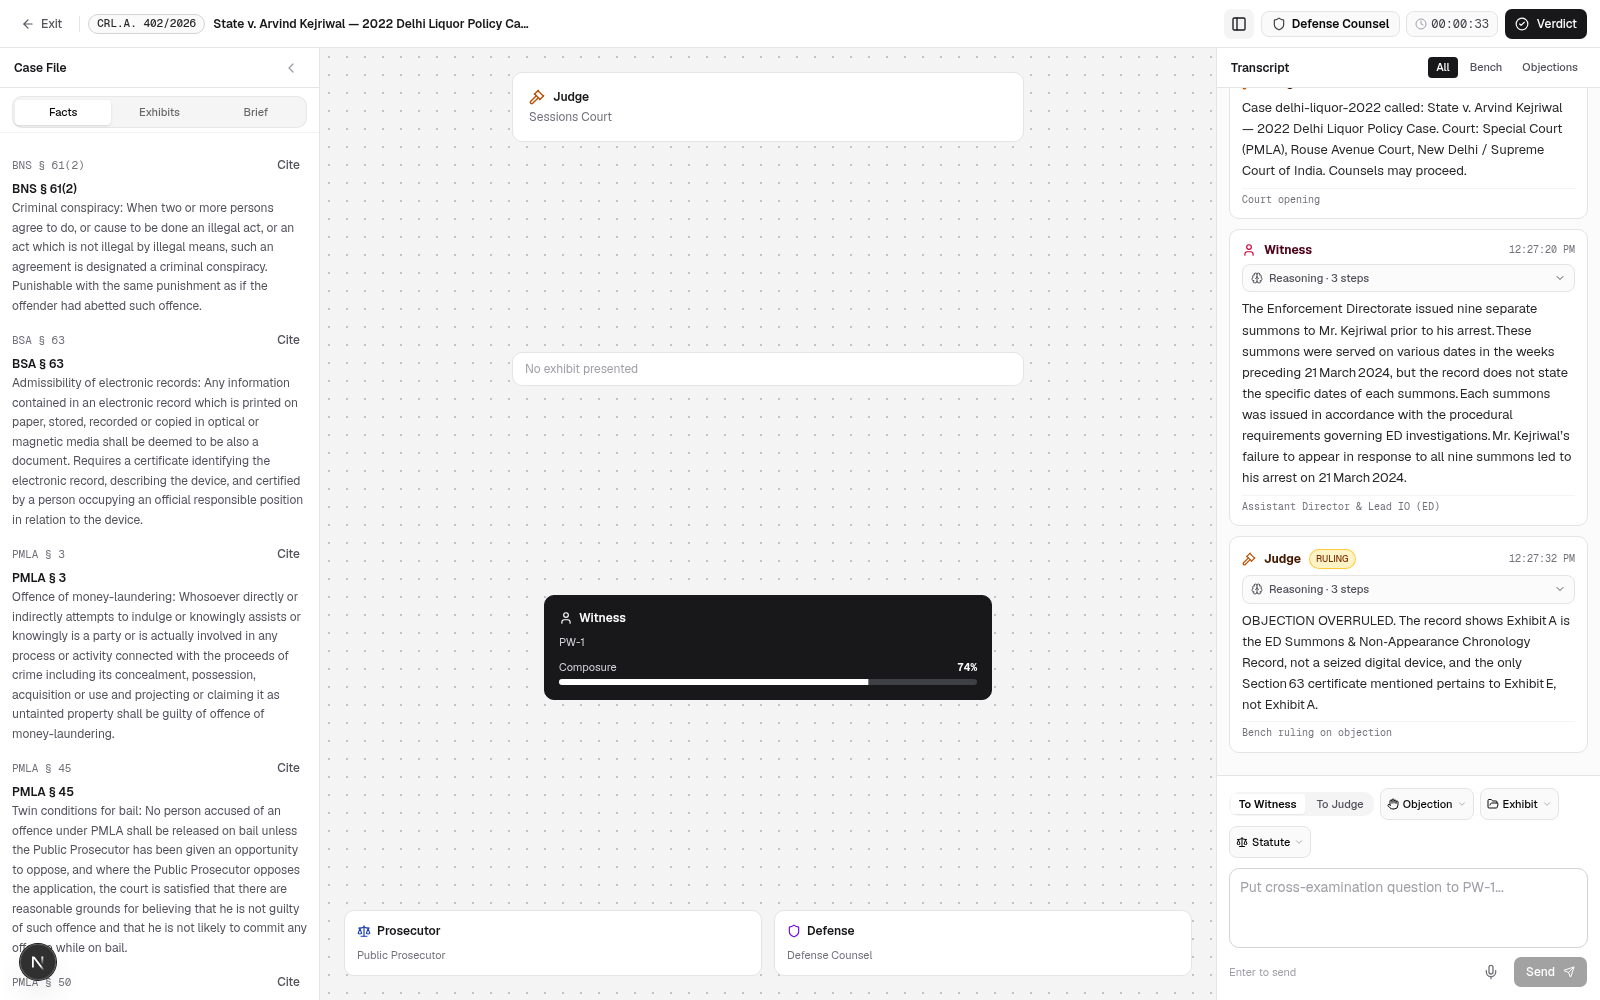
\includegraphics[width=0.98\textwidth]{figures/objection-ruling.png}
\caption{Right-panel ruling on the student's objection. The ruling distinguishes Exhibit A (the summons chronology) from the device-seizure exhibit and cites Section 63, the provision actually on record; the pre-fix version of this figure imported Section 65B of the Information Technology Act, which appears nowhere in the corpus.}
\label{fig:objection}
\end{figure}

The verdict stage translates the transcript into an educational summary instead of a legal conclusion. The score is a feedback signal that helps the learner identify weak legal accuracy, poor objection timing or an incomplete argument (Figure~\ref{fig:verdict}).

\begin{figure}[t]
\centering
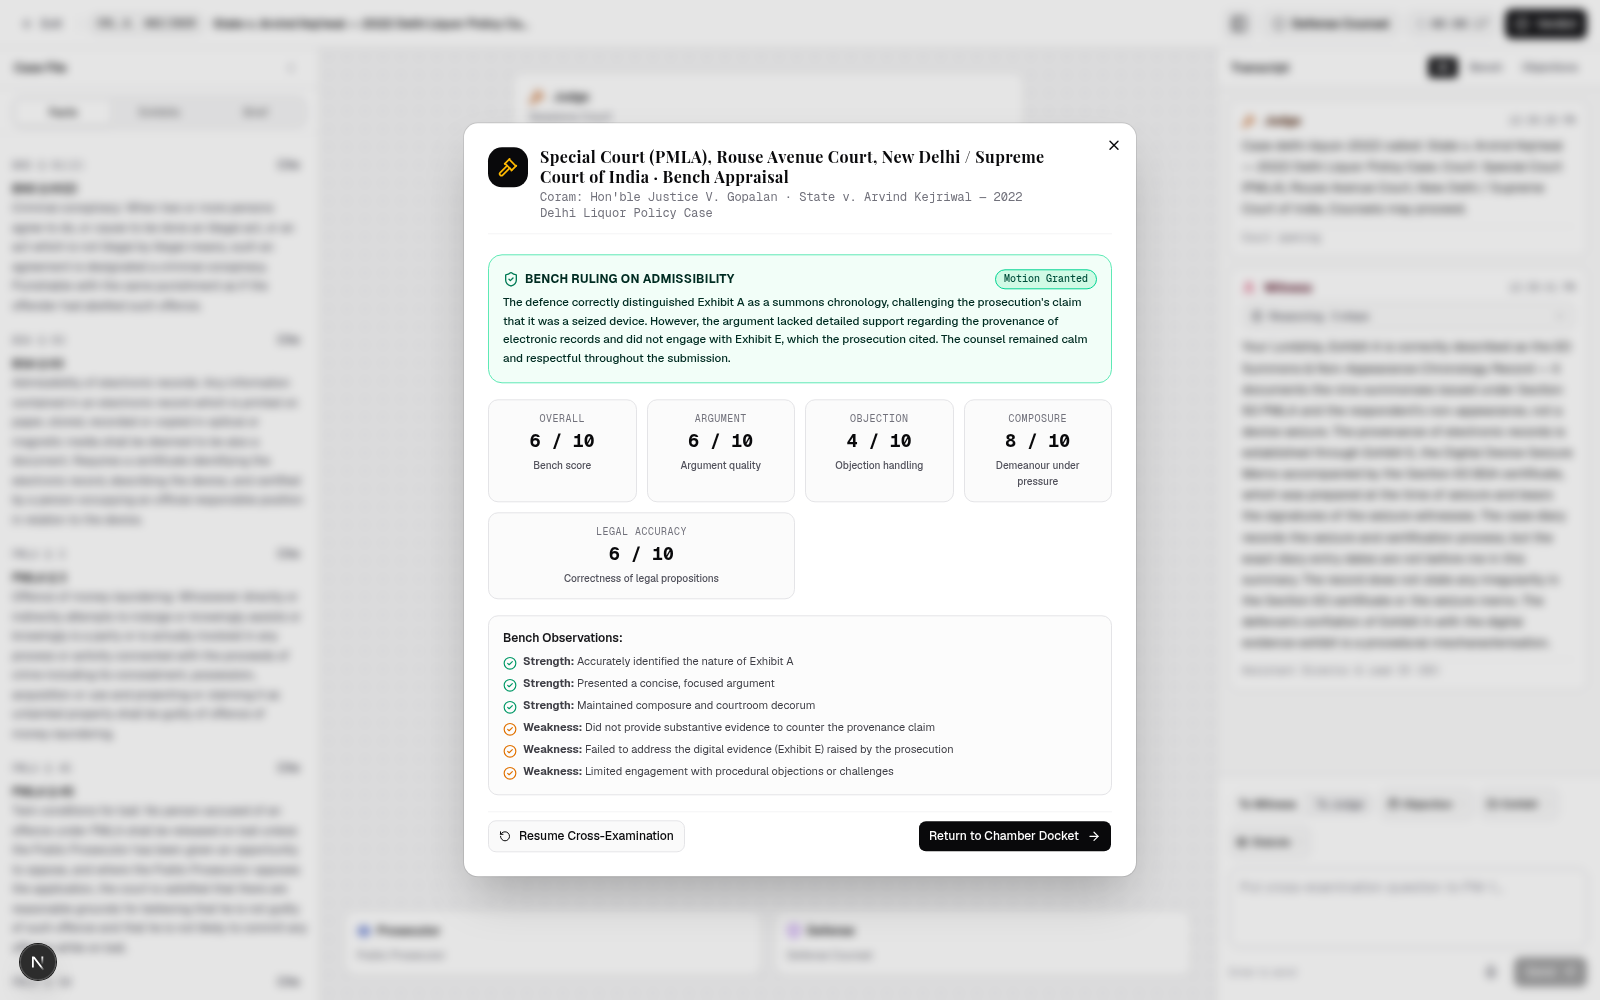
\includegraphics[width=0.98\textwidth]{figures/verdict-modal.png}
\caption{Verdict summary for the Delhi case. Scores, strengths and weaknesses for the session are shown. Bench-persona details are fictional.}
\label{fig:verdict}
\end{figure}

\subsection{Limitations}
The measured limitations of this build are as follows. Each is stated with the measurement that supports it.

\begin{itemize}
\item \textbf{Corpus size and paragraph labelling.} Only 8 of 914 chunks (0.87\%) carry an explicit ``Para $N$'' label; Bilkis and Sukanya have one each and Electoral Bonds has none. Paragraph-level relevance can therefore only be scored strictly for a subset (16 of 30 benchmark questions and 20 of 47 held-out questions); the remainder are scored at document level.
\item \textbf{Judgment chunks are shared across case pages.} Under the \texttt{case-or-null} scope a Delhi-case question may return Sita Soren, Bilkis and Sukanya chunks alongside Delhi chunks. Case-to-case isolation between the two simulation cases is verified (regression test T1), but matter-to-matter isolation is not enforced.
\item \textbf{No ANN index.} \texttt{pg\_indexes} on \texttt{chunks} contains only the primary key and the \texttt{case\_id} and \texttt{document\_id} b-trees, so every vector query is a sequential scan (measured median 96.4\,ms over 20 runs at 914 chunks). This will not hold at corpus scale.
\item \textbf{Keyword channel is weak.} The keyword-only ablation reached document-level P@5 of 0.360 (benchmark) and 0.340 (held-out) against 0.733--0.747 for the vector path.
\item \textbf{Verdict scores are not reproducible.} Five identical transcripts produced overall scores of 8, 6, 7, 5 and 7 (mean 6.6, range 5--8) even after the temperature was set to zero, because the OpenAI-compatible relay does not honour the temperature lock.
\item \textbf{Faithfulness was judged by an LLM, not a human.} 7 of 20 questions produced scoreable claims; the remaining 13 were abstentions that produced no atomic claims. A human audit of a sample is still required before the number is treated as a quality guarantee.
\item \textbf{Benchmark and held-out sets are not independent of the corpus.} All questions were authored against the same five matters the retriever searches. They measure internal consistency, not general legal-retrieval quality. The held-out set was written to avoid lexical overlap with the source passages, which is why its numbers are lower (MRR 0.936 versus 1.000 document-level).
\item \textbf{Generated answers still require human verification.} The simulator is an educational tool, not legal advice; the named parties are public-record parties in the underlying matters, while the judge, counsel and witness personas are fictional.
\end{itemize}

\section{Conclusion}
Courtroom AI demonstrates how retrieval, structured case data and streaming language-model interaction can be combined into a practical legal-education workflow. The learner begins with one of two real Indian cases, studies its facts and exhibits, asks questions grounded in the case corpus (reinforced by three verbatim 2024 Supreme Court judgments), and then enters a short timed courtroom. The learner can submit an argument, raise an objection, receive a real streamed judge or witness response on the right-side panel and finish with a rubric-based verdict report.

The implementation meets the central objectives of the mini-project: it is case-specific, persistent, interactive and verifiable through API and UI flows. The server-side duration checks complement the client timer, while source labels make RAG answers more transparent. It is also measurable: a five-cell retrieval ablation over a 30-question benchmark and a 47-question held-out set, a claim-level faithfulness judge, an eight-question not-in-corpus test, an invented-specifics scan of courtroom turns, a five-run verdict-variance test and a nine-case regression suite are all part of the repository and all report their failures as well as their passes.

Two measured results changed the design. First, the retrieval layer previously excluded every judgment chunk from case pages; after the scope fix, a Sita Soren question raised from the Delhi case page returns the Sita Soren paragraphs it should. Second, the witness and judge prompts previously permitted invention; after grounding them, a request for nine summons dates is answered with the record's own limit --- nine summons, arrest on 21 March 2024, and an explicit statement that the record does not state the individual dates. Remaining weaknesses --- paragraph labels on 0.87\% of chunks, no approximate-nearest-neighbour index, and verdict scores that vary between 5 and 8 on an identical transcript --- are stated in \S4.8 rather than smoothed over.


\subsection{Future Enhancements}
The following remain open, in the order the measurements suggest they matter.

\begin{enumerate}[label=\arabic*.]
\item \textbf{Paragraph-preserving re-ingestion.} Split the judgment text on paragraph markers instead of a sliding word window, so that every chunk carries its paragraph number. This would raise paragraph-label coverage from 8/914 to the paragraph count of the three judgments and would let the strict metric be applied to the whole question set. Cost: one re-ingest of 914 chunks plus one embedding pass at \$0.02 per million tokens.
\item \textbf{Approximate nearest-neighbour index.} Introduce \texttt{halfvec(4096)} with an HNSW index, or reduce the stored dimension, so that the sequential scan measured at 96\,ms does not become the bottleneck as the corpus grows.
\item \textbf{Question-level scope selection.} Make the scope dynamic: case chunks plus only those judgment documents whose subject the question touches, instead of all judgment chunks.
\item \textbf{Deterministic verdicts.} Replace the free-form rubric call with a scored rubric evaluated by a deterministic procedure, so that identical transcripts produce identical reports.
\item \textbf{Human-graded faithfulness sample.} Have a second reviewer label a sample of the judged claims so the LLM judge's agreement rate can be reported.
\item \textbf{Expanded corpus.} Extend from two playable cases to the ten-case corpus the project plan anticipates, ingesting further judgments and statutes through the existing pipeline.
\end{enumerate}

\section*{Appendix A: Reproducibility}
\addcontentsline{toc}{section}{Appendix A: Reproducibility}

\subsection*{A.1 Active database and images}
\begin{itemize}
\item Project: \texttt{snowy-bread-71537502} (branch \texttt{main}, \texttt{aws-ap-southeast-1})
\item Rollback branch: \texttt{pre-qwen3-backup}
\item Active schema: \texttt{vector(4096)} on \texttt{chunks.embedding}; documents: 5 rows; chunks used by retrieval: 914; embedding backfill verified complete by \texttt{SELECT count(*) FROM chunks WHERE embedding IS NULL} returning 0.
\item Embedding model: \texttt{qwen/qwen3-embedding-8b} via OpenRouter; generation class: cloud, not local CPU.
\end{itemize}

\subsection*{A.2 Environment variables expected (names only, values are secret)}
\begin{itemize}
\item Database: \texttt{DATABASE\_URL}, \texttt{DATABASE\_URL\_UNPOOLED}
\item Neon branch: \texttt{NEON\_BRANCH}, \texttt{NEON\_BRANCH\_ID}, \texttt{NEON\_FUNCTION\_HOST\_SUFFIX}
\item Auth: \texttt{NEON\_AUTH\_BASE\_URL}, \texttt{NEON\_AUTH\_COOKIE\_SECRET}, \texttt{NEON\_AUTH\_JWKS\_URL}
\item Gateway: \texttt{NEON\_AI\_GATEWAY\_BASE\_URL}, \texttt{NEON\_AI\_GATEWAY\_TOKEN}
\item Providers: \texttt{GROQ\_API\_KEY}, \texttt{OPENROUTER\_API\_KEY}
\item Misc: \texttt{FIRECRAWL\_API\_KEY}, \texttt{HF\_TOKEN}, \texttt{NEXT\_PUBLIC\_APP\_URL}
\end{itemize}

\subsection*{A.3 Scripts used in the migration}
\begin{itemize}
\item \texttt{extract-judgments.mjs} --- PDF to JSON extraction of the three 2024 judgments from public Supreme Court PDFs.
\item \texttt{ingest-judgments.mjs} --- canonicalises judgment text, chunks \texttt{judgment} documents and inserts \texttt{chunks} rows.
\item \texttt{migrate-embeddings.mjs} --- alters schema to \texttt{vector(4096)}, nulls legacy embeddings, re-embeds through OpenRouter.
\item \texttt{run-legal-eval.mjs} --- 30-question retrieval benchmark across the five matters; writes the JSON report.
\item \texttt{backfill-embeddings.mjs} --- generic NULL-embedding backfill with \texttt{BATCH\_SIZE} and \texttt{LIMIT} controls.
\item \texttt{eval-rag.mjs} --- earlier harness (20-question subset, hybrid weights), superseded by \texttt{run-legal-eval.mjs}.
\item \texttt{ablation-gold.mts} --- current five-cell ablation with document-level and gold-chunk metrics over the benchmark and held-out sets; writes \texttt{data/eval/ablation\_gold.json}.
\item \texttt{build-gold-chunks.mts} --- builds \texttt{data/eval/gold\_chunks.json}: the gold chunk identifiers per question, and the list of questions whose gold target could not be found.
\item \texttt{prefix-ab.mts} --- A/B test of the qwen3 query-instruction prefix.
\item \texttt{eval-faithfulness.mts} --- claim-level LLM-judge faithfulness with abstention classification; writes \texttt{data/eval/faithfulness.json}.
\item \texttt{not-in-corpus.mts} --- eight questions whose answers are absent from the corpus; records whether the system abstains, hedges or invents.
\item \texttt{regression-tests.mjs} --- nine end-to-end regression tests over the live API.
\end{itemize}

\subsection*{A.4 Commands}
{\footnotesize
\begin{verbatim}
cd report
pdflatex CourtroomAI_MiniProject_Report.tex
pdflatex CourtroomAI_MiniProject_Report.tex
node scripts/regression-tests.mjs                 # regression suite
node --experimental-strip-types scripts/ablation-gold.mts
node --experimental-strip-types scripts/build-gold-chunks.mts
node --experimental-strip-types scripts/eval-faithfulness.mts
node --experimental-strip-types scripts/prefix-ab.mts
node --experimental-strip-types scripts/not-in-corpus.mts
node scripts/measure-latency.mjs
\end{verbatim}
}

\subsection*{A.4a Regression suite output (verbatim)}
Captured with \texttt{node scripts/regression-tests.mjs} against the running application. The T5 event list is abbreviated here; the full sequence is reasoning, then many delta events, then a final \texttt{done} event.
{\footnotesize
\begin{verbatim}
PASS  T1 case-scope isolation
PASS  T0 session create 201
PASS  T2a intro ok 201
PASS  T2b verdict ends session (and parse)
PASS  T2c intro on ended session -> 409
FAIL  T3 wrong owner -- skipped -- needs two auth users;
      no DB write allowed
PASS  T4 intro on missing session -> 404
PASS  T5 stream emits done event
PASS  T6 verdict schema valid
PASS  T7 source labels non-empty
9 tests ran, 0 failed
\end{verbatim}
}

\subsection*{A.5 Claims that could not be re-verified}
\begin{itemize}
\item The \texttt{pre-qwen3-backup} rollback integrity was not re-verified from scratch; it is a Neon branch created on the live project and assumed intact.
\item Regression test T3 (wrong-owner access) was \emph{skipped}: proving it needs two authenticated users, which would require a database write that was not authorised for this task.
\item The faithfulness harness depends on an LLM judge from the same vendor as the generator, and 13 of 20 questions produced no scoreable claims; the reported 77\% therefore rests on 7 questions and 31 claims, not on the full set.
\item The earlier hybrid numbers in \texttt{data/eval-results.json} are from a pre-migration 20-question run and are superseded by \texttt{data/eval/ablation\_gold.json}.
\item Benchmarks were run on a derived corpus whose questions were authored against the five matters. They do not constitute a general-purpose legal-retrieval leaderboard result, and the held-out set was written by the same pipeline.
\item \texttt{pre-qwen3-backup} contents were not compared chunk-by-chunk against the migrated branch.
\end{itemize}

\begin{thebibliography}{9}
\bibitem{rag} P. Lewis et al., ``Retrieval-Augmented Generation for Knowledge-Intensive NLP Tasks,'' \emph{Advances in Neural Information Processing Systems}, 2020.
\bibitem{nextjs} Vercel, ``Next.js Documentation: App Router and Route Handlers,'' 2026.
\bibitem{postgres} Neon, ``Neon Serverless Postgres Documentation,'' 2026.
\bibitem{electoral} Association for Democratic Reforms v. Union of India, 2024 INSC 113, Supreme Court of India.
\bibitem{liquor} Directorate of Enforcement and Central Bureau of Investigation proceedings concerning the 2021--22 Delhi Excise Policy, public case records, 2022--2024.
\bibitem{bsa} The Bharatiya Sakshya Adhiniyam, 2023, provisions concerning electronic records.
\bibitem{pmla} The Prevention of Money-Laundering Act, 2002, Section 3.
\bibitem{groq} Groq, ``OpenAI-Compatible Chat Completions and Streaming API,'' 2026.
\bibitem{soren} Sita Soren v. Union of India, 2024 INSC 161, Supreme Court of India (seven-judge Bench).
\bibitem{bilkis} Bilkis Yakub Rasool v. Union of India, 2024 INSC 24, Supreme Court of India.
\bibitem{sukanya} Sukanya Shantha v. Union of India, 2024 INSC 753, Supreme Court of India.
\bibitem{qwen} Y. Zhang, M. Li, D. Long, X. Zhang, H. Lin et al. \texttt{Qwen3 Embedding: Advancing Text Embedding and Reranking Through Foundation Models}. arXiv:2506.05176, 2025.
\bibitem{indiclegalqa} Pandey et al., ``Dataset for legal question answering system in the Indian judiciary context,'' \emph{Data in Brief} 60 (2025) 111647. DOI: 10.17632/gf8n8cnmvc.2.
\end{thebibliography}
\end{document}
